\chapter{Recursive Data Types}\label{recursive_data_chap}

\emph{Recursive data types}%
\index{recursive data type|textbf}
%\index{recursive data type|seealso{induction}} 
play a central role in programming, and induction is really all about them.

Recursive data types are specified by \emph{recursive definitions},
which say how to construct new data elements from previous ones.
Along with each recursive data type there are recursive definitions of
properties or functions on the data type.  Most importantly, based on
a recursive definition, there is a \emph{structural induction}%
\index{induction!structural induction}
method for proving that all data of the given type have some property.

This chapter examines a few examples of recursive data types and
recursively defined functions on them:
\begin{itemize}
\item strings of characters,
\item ``balanced'' strings of brackets,
\item the nonnegative integers, and
\item arithmetic expressions.
\item two-player games with perfect information.
\end{itemize}

%\hyperdef{paren}{string}
\section{Recursive Definitions and Structural Induction}

We'll start off illustrating recursive definitions and proofs using
the example of character strings.  Normally we'd take strings of
characters for granted, but it's informative to treat them as a
recursive data type.  In particular, strings are a nice first example
because you will see recursive definitions of things that are easy to
understand, or that you already know, so you can focus on how the
definitions work without having to figure out what they are supposed
to mean.

Definitions of recursive data types have two parts:
\begin{itemize}
\item \inductioncase{Base case(s)} specifying that some known
  mathematical elements are in the data type, and
\index{base case|see{recursive data type}}

\item \inductioncase{Constructor case(s)} that specify how to construct new data
  elements from previously constructed elements or from base elements.
\end{itemize}

The definition of strings over a given character set $A$ follows this
pattern:

\begin{definition}\label{recstring_def}
  Let $A$ be a nonempty set called an \emph{alphabet}, whose elements
  are referred to as \emph{characters} (also called \emph{letters},
  \emph{symbols}, or \emph{digits}).  The recursive data type
  $\strings{A}$ of strings over alphabet $A$ is defined as follows:
\begin{itemize}
\item \inductioncase{Base case}: the empty string $\emptystring$ is in $\strings{A}$.

\item \inductioncase{Constructor case}: If $a \in A$ and $s \in \strings{A}$, then the pair
       $\ang{a,s} \in \strings{A}$.
\end{itemize}
\end{definition}
So $\strings{\set{0,1}}$ are the binary strings.

The usual way to treat binary strings is as sequences of 0's and 1's.
For example, we have identified the length-4 binary string 1011 as a
sequence of bits, the 4-tuple $(1,0,1,1)$.  But according to
the recursive Definition~\ref{recstring_def}, this string would be
represented by nested pairs, namely
\[
\ang{1,\ang{0,\ang{1,\ang{1,\emptystring}}}}.
\]
These nested pairs are definitely cumbersome and may also seem
bizarre, but they actually reflect the way that such lists of
characters would be represented in programming languages like Scheme
or Python, where $\ang{a,s}$ would correspond to $\text{cons}(a, s)$.

Notice that we haven't said exactly how the empty string is
represented.  It really doesn't matter, as long as we can recognize
the empty string and not confuse it with any nonempty string.

\begin{editingnotes}
Even before func def, define binary relation def, say ``$t$ a proper
suffix of $s''$ or ``$t$ is a subsequence of $s$'' and then set up
func def as special case
\end{editingnotes}

Continuing the recursive approach, let's define the length of a string.
\begin{definition}
The length $\lnth{s}$ of a string $s$ is defined recursively based
on Definition~\ref{recstring_def}.

\item \inductioncase{Base case}:  $\lnth{\emptystring} \eqdef\ 0$.

\item \inductioncase{Constructor case}: $\lnth{\ang{a,s}} \eqdef\ 1 + \lnth{s}$.

\end{definition}

This definition of length follows a standard pattern: functions on
recursive data types can be defined recursively using the same cases
as the data type definition.  Specifically, to define a function $f$
on a recursive data type, define the value of $f$ for the base cases
of the data type definition, then define the value of $f$ in each
constructor case in terms of the values of $f$ on the component data
items.

Let's do another example: the \emph{concatenation} $s\cdot t$ of the
strings $s$ and $t$ is the string consisting of the letters of $s$
followed by the letters of $t$.  This is a perfectly clear
mathematical definition of concatenation (except maybe for what to do
with the empty string), and in terms of Scheme/Python lists, $s\cdot
t$ would be the list $\text{append}(s, t)$.  Here's a recursive
definition of concatenation.

\begin{definition}\label{concat_def}
The \term{concatenation} $s\cdot t$ of the strings $s,t \in
\strings{A}$ is defined recursively based on
Definition~\ref{recstring_def}:

\item \inductioncase{Base case}:     % ($s=\emptystring$):
\[
\emptystring \cdot t \eqdef\ t.
\]

\item \inductioncase{Constructor case}: %($s = \ang{a,r}$ for $r \in \strings{A}$):
\[
\ang{a,s} \cdot t \eqdef\ \ang{a, s \cdot t}.
\]
\end{definition}

\subsection{Structural Induction}

\emph{Structural induction}%
\index{induction!structural induction|textbf} 
is a method for proving that all the elements
of a recursively defined data type have some property.  A structural
induction proof has two parts corresponding to the recursive definition:
\begin{itemize}
\item Prove that each base case element has the property.
\item Prove that each constructor case element has the property, when
  the constructor is applied to elements that have the property.
\end{itemize}

For example, in the base case of the definition of
concatenation~\ref{concat_def}, we \emph{defined} concatenation so the empty
string was a ``left identity,'' namely, $\emptystring \cdot s\ \eqdef s$.  We
intend the empty string also to be a ``right identity,'' namely, $s \cdot
\emptystring = s$.  Being a right identity is not part of
Definition~\ref{concat_def}, but we can prove it easily by structural induction:
\begin{lemma}\label{rightidempty}
\[
s \cdot \emptystring = s
\]
for all $s \in \strings{A}$.
\end{lemma}

\begin{proof}
The proof is by structural induction on the recursive
definition~\ref{concat_def} of concatenation.  The induction
hypothesis will be
\[
P(s) \eqdef\ [s \cdot \emptystring = s].
\]

\inductioncase{Base case}: ($s = \emptystring$).
\begin{align*}
s \cdot \emptystring
    & = \emptystring \cdot \emptystring\\
    & = \emptystring
        & \text{($\emptystring$ is a left identity by Def~\ref{concat_def})}\\
    & = s.
\end{align*}

\inductioncase{Constructor case}: ($s = \ang{a,t}$).
\begin{align*}
s \cdot \emptystring
   & = \ang{a,t} \cdot \emptystring\\
   & \eqdef\ \ang{a, t \cdot \emptystring}.
       & \text{(Constructor case of Def~\ref{concat_def})}\\
   & = \ang{a,t}
        & \text{by induction hypothesis $P(t)$}\\
   & = s.
\end{align*}
So $P(s)$ holds.  This completes the proof of the constructor case,
and we conclude by structural induction that
equation~\eqref{rightidempty} holds for all $s \in \strings{A}$.
\end{proof}

We can also verify properties of recursive functions by structural
induction on their definitions.  For example, let's verify the
familiar fact that the length of the concatenation of two strings is
the sum of their lengths:

%\begin{theorem}\label{stAl+}
%\end{theorem}
\begin{lemma*}
\[
\lnth{s\cdot t} = \lnth{s} + \lnth{t}
\]
for all $s,t \in \strings{A}$.
\end{lemma*}

\begin{proof}
By structural induction on the definition of $s \in \strings{A}$.   The
induction hypothesis is
\[
P(s) \eqdef\ \forall t \in \strings{A}.\, \lnth{s\cdot t} = \lnth{s} + \lnth{t}.
\]

\inductioncase{Base case} ($s = \emptystring$):
\begin{align*}
\lnth{s \cdot t}
   & = \lnth{\emptystring \cdot t}\\
   & = \lnth{t}
         & \text{(base case of Def~\ref{concat_def} of concatenation)}\\
   & = 0 + \lnth{t}\\
   & = \lnth{s} + \lnth{t}
         & \text{(Def of $\lnth{\emptystring}$)}.
\end{align*}

\inductioncase{Constructor case}: ($s \eqdef \ang{a,r}$).
\begin{align*}
\lnth{s \cdot t}
    & = \lnth{\ang{a, r} \cdot t}\\
    & = \lnth{\ang{a,r \cdot t}}
        &  \text{(constructor case of Def of concat)}\\
    & = 1 + \lnth{r \cdot t}
        &  \text{(constructor case of def length)}\\
    & = 1 +  (\lnth{r} + \lnth{t})
        & \text{(ind. hyp. $P(r)$)}\\
    & = (1 +  \lnth{r}) + \lnth{t}\\
    & = \lnth{\ang{a,r}} + \lnth{t}
        & \text{(constructor case, def of length)}\\
    & = \lnth{s} + \lnth{t}.
\end{align*}
This proves that $P(s)$ holds, completing the constructor case.  By
structural induction, we conclude that $P(s)$ holds for all strings $s
\in \strings{A}$.
\end{proof}

These proofs illustrate the general principle:

\textbox{ 
\textboxtitle{The Principle of Structural Induction.}

Let $P$ be a predicate on a recursively defined data type $R$.  If
%
\noindent \begin{itemize}
\item $P(b)$ is true for each base case element $b \in R$, and

\item for all two-argument constructors $\mathbf{c}$,
\[
[P(r)\QAND P(s)] \QIMPLIES P(\mathbf{c}(r, s))
\]
for all $r,s \in R$,\\
and likewise for all constructors taking other numbers of arguments,
\end{itemize}
then
\[
P(r) \text{ is true for all } r \in R.
\]
}

\begin{problems}
\practiceproblems
\pinput{FP_binary_tree_induction}

\classproblems
\pinput{CP_string_associativity}
\pinput{CP_string_reversal}
\pinput{CP_F18_functions}
\pinput{CP_recursively_defined_sets}
\pinput{CP_binary_trees}

\homeworkproblems
%\pinput{PS_string_cancellation}
\pinput{PS_palindromes}
\pinput{PS_linear_combination_by_structural_induction}
\pinput{PS_count_a_s_lem}
\pinput{PS_koch_snowflake}
\pinput{PS_red_black_tree_induction}

\examproblems
\pinput{FP_arith_trig_functions}
\pinput{FP_structural_induction_rational_composition_s16}
\pinput{FP_structural_linear_product}
\pinput{FP_recstrings}

%%%%\pinput{CP_recursive_binary_trees}  %%problem idea, needs work.
\end{problems}

\section{Strings of Matched Brackets}

Let $\brkts$ be the set of all strings of square brackets.  For example,
the following two strings are in $\brkts$:
\begin{equation}\label{2strings}
\lefbrk\rhtbrk\rhtbrk\lefbrk\lefbrk\lefbrk\lefbrk\lefbrk\rhtbrk\rhtbrk\quad \text{and}\quad \lefbrk\lefbrk\lefbrk\rhtbrk\rhtbrk\lefbrk\rhtbrk\rhtbrk\lefbrk\rhtbrk
\end{equation}

A string $s \in \brkts$ is called a \emph{matched string} if its
brackets ``match up'' in the usual way.  For example, the left-hand
string above is not matched because its second right bracket does not
have a matching left bracket.  The string on the right is matched.

We're going to examine several different ways to define and prove
properties of matched strings using recursively defined sets and
functions.  These properties are pretty straightforward, and you might
wonder whether they have any particular relevance in computer science.
The honest answer is ``not much relevance \emph{any more}.''  The reason
for this is one of the great successes of computer science, as explained in
the text box below.

\textbox{
\textboxheader{Expression Parsing}
%Flesh this out and get references

During the early development of computer science in the 1950's and 60's,
creation of effective programming language compilers was a central
concern.  A key aspect in processing a program for compilation was
expression parsing.  One significant problem was to take an expression
like
\[
x + y * z^2 \div y + 7
\]
and \emph{put in} the brackets that determined how it
should be evaluated---should it be
\begin{align*}
[[x + y] * z^2 \div y] + 7,\text{ or}, \\
x + [y * z^2 \div [y + 7]], \text{ or},\\
[x + [y * z^2 ]] \div [y + 7], \text{ or}\dots?
\end{align*}

The Turing award (the ``Nobel Prize'' of computer science) was
ultimately bestowed on Robert W. Floyd,%
\index{Floyd, Robert W.} 
for, among other things,
discovering simple procedures that would insert the brackets properly.

In the 70's and 80's, this parsing technology was packaged into high-level
compiler-compilers that automatically generated parsers from expression
grammars.  This automation of parsing was so effective that the subject no
longer demanded attention.  It had largely disappeared from the computer
science curriculum by the 1990's.}

\iffalse
One precise way to determine if a string is matched is to start with 0 and
read the string from left to right, adding 1 to the count for each left
bracket and subtracting 1 from the count for each right bracket.
For example, here are the counts for the two strings above
\[\begin{array}{rrrrrrrrrrrrr}
& \lefbrk & \rhtbrk & \rhtbrk & \lefbrk & \lefbrk & \lefbrk & \lefbrk &
\lefbrk & \rhtbrk & \rhtbrk & \rhtbrk & \rhtbrk\\
0 & 1 & 0 & -1 & 0 & 1 & 2 & 3 & 4 & 3 & 2 & 1 & 0\\
\\
\\
& \lefbrk & \lefbrk & \lefbrk & \rhtbrk & \rhtbrk & \lefbrk & \rhtbrk &
\rhtbrk & \lefbrk & \rhtbrk\\
0 & 1 & 2 & 3 & 2 & 1 & 2 & 1 & 0 & 1 & 0
\end{array}\]
A string has a \emph{good count} if its running count never goes
negative and ends with 0.  So the second string above has a good count, but
the first one does not because its count went negative at the third step.
\begin{definition}\label{gc-def}
Let
\[
\GC \eqdef\  \set{ s \in \brkts \suchthat s\ \text{has a good count}}.
\]
\end{definition}
The matched strings can now be characterized precisely as this set of
strings with good counts.
\fi

The matched strings can be nicely characterized as a recursive data type:

\begin{definition}\label{RM_def}\label{RM-def}
Recursively define the set $\RM$ of strings as follows:
\begin{itemize}

\item \inductioncase{Base case}: $\emptystring \in\RM$.

\item \inductioncase{Constructor case}: If $s,t \in\RM$, then
\[
\lefbrk s\, \rhtbrk t \in \RM.
\]
\end{itemize}

\end{definition}

Here $\lefbrk s\, \rhtbrk t$ refers to the concatenation of
strings which would be written in full as
\[
\lefbrk \cdot (s \cdot (\rhtbrk \cdot t)).
\]
From now on, we'll usually omit the ``$\cdot$'s.'' 

Using this definition, $\emptystring \in\RM$ by the base
case, so letting $s=t =\emptystring$ in the constructor case implies
\[
\lefbrk\emptystring\rhtbrk\emptystring=\lefbrk\rhtbrk\in\RM.
\]
Now,
\begin{align*}
\lefbrk\emptystring\rhtbrk\lefbrk\rhtbrk &= \lefbrk\rhtbrk\lefbrk\rhtbrk \in \RM
    & \text{(letting $s = \emptystring, t = \lefbrk\rhtbrk$)}\\
\lefbrk\lefbrk\rhtbrk\rhtbrk\emptystring & = \lefbrk\lefbrk\rhtbrk\rhtbrk \in \RM
    & \text{(letting $s = \lefbrk\rhtbrk, t = \emptystring$)}\\
&\ \ \lefbrk\lefbrk\rhtbrk\rhtbrk\lefbrk\rhtbrk \in \RM
    & \text{(letting $s = \lefbrk\rhtbrk, t = \lefbrk\rhtbrk$)}
\end{align*}
are also strings in $\RM$ by repeated applications of the constructor
case; and so on.

\iffalse
If you haven't seen this kind of definition before, you should
try continuing this example to verify that
$\lefbrk\lefbrk\lefbrk\rhtbrk\rhtbrk\lefbrk\rhtbrk\rhtbrk\lefbrk\rhtbrk
\in \RM$.
\fi


\iffalse
Given the way this section is set up you might guess that $\RM = \GC$,
and you'd be right, but it's not completely obvious.  The proof is worked
out in Problem~\ref{PS_bracket_good_count}.
\fi

It's pretty obvious that in order for brackets to match, there had
better be an equal number of left and right ones.  For further
practice, let's carefully prove this from the recursive definitions,
beginning with a recursive definition of the number $\cnt{c}{s}$ of
occurrences of the character $c \in A$ in a string $s$:

\begin{definition}\label{countas_def} \mbox{}

\inductioncase{Base case}: $\cnt{c}{\emptystring} \eqdef\ 0$.

\inductioncase{Constructor case}:
\[
\cnt{c}{\ang{a,s}} \eqdef \begin{cases}
                           \cnt{c}{s}  &\text{ if } a \neq c,\\
                           1 + \cnt{c}{s} &\text{ if } a = c.
                           \end{cases}
\]
\end{definition}

The following Lemma follows directly by structural induction on
Definition~\ref{countas_def}.  We'll leave the proof for practice
(Problem~\ref{PS_count_a_s_lem}).

\begin{lemma}\label{countas_lem}
\[
\cnt{c}{s \cdot t} = \cnt{c}{s} + \cnt{c}{t}.
\]
\end{lemma}

\begin{lemma*}
Every string in $\RM$ has an equal number of left and right brackets.

\begin{proof}
The proof is by structural induction with induction hypothesis
\[
P(s) \eqdef\  \brac{\cnt{\lefbrk}{s} = \cnt{\rhtbrk}{s}}.
\]

\inductioncase{Base case}: $P(\emptystring)$ holds because
\[
\cnt{\lefbrk}{\emptystring} = 0 = \cnt{\rhtbrk}{\emptystring}
\]
by the base case of Definition~\ref{countas_def} of $\cnt{c}{}$.

\inductioncase{Constructor case}: By structural induction hypothesis, we assume
$P(s)$ and $P(t)$ and must show $P(\lefbrk s\,\rhtbrk t)$:
\begin{align*}
\cnt{\lefbrk}{\lefbrk s\,\rhtbrk t}
    & = \cnt{\lefbrk}{\lefbrk} + \cnt{\lefbrk}{s}
        +\cnt{\lefbrk}{\rhtbrk}+ \cnt{\lefbrk}{t}
         & \text{(Lemma~\ref{countas_lem})}\\
    & = 1 + \cnt{\lefbrk}{s} + 0 + \cnt{\lefbrk}{t}
         & \text{(def $\cnt{\lefbrk}{}$)}\\
    & = 1 + \cnt{\rhtbrk}{s} + 0 + \cnt{\rhtbrk}{t}
         & \text{(by $P(s)$ and $P(t)$)}\\
    & = 0 + \cnt{\rhtbrk}{s} + 1 + \cnt{\rhtbrk}{t}\\
    & = \cnt{\rhtbrk}{\lefbrk} + \cnt{\rhtbrk}{s}
        +\cnt{\rhtbrk}{\rhtbrk}+ \cnt{\rhtbrk}{t}
         & \text{(def $\cnt{\rhtbrk}{}$)}\\
    & = \cnt{\rhtbrk}{\lefbrk s\,\rhtbrk t}
            & \text{(Lemma~\ref{countas_lem})}
\end{align*}
This completes the proof of the constructor case.  We conclude by
structural induction that $P(s)$ holds for all $s \in\RM$.
\end{proof}
\end{lemma*}

\iffalse

The \term{depth} of a matched string is defined recursively as follows
\begin{definition}
The \emph{depth} $d(s)$ of a string $s \in\RM$ is defined
recursively by the rules:
\begin{itemize}
\item $d(\emptystring) \eqdef\  0.$
\item $d(\lefbrk s\,\rhtbrk t)
    \eqdef\ \max \set{d(s) + 1, d(t)}$
\end{itemize}
\end{definition}
\fi

\textbf{Warning:}%
\index{recursive data type!ambiguity} 
When a recursive definition of a data type allows
the same element to be constructed in more than one way, the
definition is said to be \emph{ambiguous}.  We were careful to choose
an \emph{un}ambiguous definition of $\RM$ to ensure that functions
defined recursively on its definition would always be well-defined.
Recursively defining a function on an ambiguous data type
definition usually will not work.  To illustrate the problem, here's
another definition of the matched strings.

\iffalse Recursive definitions of tagged data types, where the tag
uniquely determines the rule used to construct an element, are guaranteed
to be unambiguous.
\fi

\begin{definition}\label{AM_def}
Define the set, $\AM \subseteq \brkts$ recursively as follows:
\begin{itemize}

\item \inductioncase{Base case}: $\emptystring \in \AM$,

\item \inductioncase{Constructor cases}: if $s,t \in \AM$, then
  the strings $\lefbrk s\, \rhtbrk$ and $st$ are also in $\AM$.
\end{itemize}
\end{definition}

It's pretty easy to see that the definition of $\AM$ is just another
way to define $\RM$, that is $\AM = \RM$ (see
Problem~\ref{PS_RM_equal_AM}).  The definition of $\AM$ is arguably
easier to understand, but we didn't use it because it's ambiguous,
while the trickier definition of $\RM$ is unambiguous.  Here's an
example that illustrates why this matters.  Let's define the number of
operations $f(s)$ to construct a matched string $s$ recursively on the
definition of $s \in \AM$:
\begin{align*}
  f(\emptystring)        & \eqdef\ 0, \tag{$f$ base case}\\
  f(\lefbrk s\,\rhtbrk\ ) & \eqdef\ 1+ f(s), \\
  f(st)                  & \eqdef\ 1+ f(s) +f(t).\tag{$f$ concat case}
\end{align*}
This definition may seem ok, but it isn't:
$f(\emptystring)$ winds up with two values, and consequently:
\begin{align*}
0 & = f(\emptystring) & \text{($f$ base case))}\\
  & = f(\emptystring \cdot \emptystring) & \text{(concat def, base case)} \\
                & = 1 + f(\emptystring) + f(\emptystring)
                      &  \text{($f$ concat case)},\\
                & = 1 + 0 + 0 = 1
                      & \text{($f$ base case)}.
\end{align*}
This is definitely not a situation we want to be in!

\begin{problems}

\practiceproblems
\pinput{MQ_recursive_power5}
\pinput{MQ_RM_subs_M}
%\pinput{MQ_ambiguous_recursive_def}

\classproblems
\pinput{CP_erasable_strings}
\pinput{PS_RM_equal_AM}

\homeworkproblems
\pinput{PS_bracket_good_count}
\pinput{CP_triangle_tiling_recursive}
\pinput{PS_starfree_recursive}
\pinput{PS_circuit_data_type}

\examproblems
\pinput{CP_XOR_AND_recursive}
\end{problems}

\section{Recursive Functions on Nonnegative Integers}

The nonnegative integers can be understood as a recursive data type.
\begin{definition}\label{0succ}
The set $\nngint$ is a data type defined recursively as:
\begin{itemize}
\item $0 \in \nngint$.
\item If $n \in \nngint$, then the \emph{successor} $n+1$ of $n$ is in
$\nngint$.
\end{itemize}

\end{definition}

The point here is to make it clear that ordinary induction is simply the
special case of structural induction on the recursive
Definition~\ref{0succ}.  This also justifies the familiar recursive
definitions of functions on the nonnegative integers.

\subsection{Some Standard Recursive Functions on $\nngint$}

\begin{example}\label{factorial-def}

\emph{The factorial%
\index{factorial|textbf} function.}  This function is often written
``$n!$.''  You will see a lot of it in later chapters.  Here, we'll use
the notation $\text{fac}(n)$:
\begin{itemize}
\item $\text{fac}(0) \eqdef 1$.
\item $\text{fac}(n+1) \eqdef (n+1)\cdot \text{fac}(n)$ for $n \ge 0$.
\end{itemize}
\end{example}

\begin{example}
\emph{Summation notation.}\label{sum-notation-def}\index{summation notation} Let 
``$S(n)$'' abbreviate the expression ``$\sum_{i=1}^n f(i)$.''  We can recursively define
$S(n)$ with the rules
  \begin{itemize}
  \item $S(0) \eqdef 0$.
  \item $S(n+1) \eqdef  f(n+1) + S(n)$ for $n\geq 0$.
  \end{itemize}
\end{example}

\begin{editingnotes}

\item[Simultaneous recursive definitions:]
  You can define several things at the same time, in terms of each
  other.  For example, we may define two functions $f$ and $g$ from
  $\nngint$ to $\nngint$, recursively, by:
  \begin{itemize}
  \item
    $f(0) \eqdef 1$,
  \item
    $g(0) \eqdef 1$,
  \item
    $f(n+1) \eqdef f(n) + g(n)$, for $n \geq 0$,
  \item
    $g(n+1) \eqdef f(n) \cdot g(n)$, for $n \geq 0$.
  \end{itemize}

\end{editingnotes}

\begin{editingnotes}

\subsection{Induction on Fibonacci Numbers}

We can use the recursive definition of a function to establish its
properties by structural induction.

As an illustration, we'll prove a cute identity involving Fibonacci
numbers.  Fibonacci numbers provide lots of fun for mathematicians because
they satisfy many such identities.
\begin{proposition}
\[
\forall n \geq 0 (\Sigma_{i=0}^n F_i^2 = F_n F_{n+1}).
\]
\end{proposition}

Example: $n = 4$:
\[
0^2 + 1^2 + 1^2 + 2^2 + 3^2 = 15 = 3 \cdot 5.
\]
Let's try a proof by (ordinary, not strong) induction.  The theorem
statement suggests trying it with $P(n)$ defined as:
\[
\sum_{i=0}^n F_i^2 = F_n F_{n+1}.
\]

\inductioncase{Base case} ($n=0$):
$\Sigma_{i=0}^0 F_i^2 \eqdef (F_0)^2 = 0 = F_0 F_1$ because
$F_0 \eqdef 0$.

\inductioncase{Inductive step} ($n\geq 0$): Now we stare at the gap
between $P(n)$ and $P(n+1)$.  $P(n+1)$ is given by a summation that's
obtained from that for $P(n)$ by adding one term; this suggests that,
once again, we subtract.  The difference is just the term $F_{n+1}^2$.
Now, we are assuming that the original $P(n)$ summation totals $F_n
F_{n+1}$ and want to show that the new $P(n+1)$ summation totals
$F_{n+1} F_{n+2}$.  So we would \emph{like} the difference to be
\[
F_{n+1} F_{n+2} - F_n F_{n+1}.
\]

So, the actual difference is $F_{n+1}^2$ and the difference we want is
$F_{n+1} F_{n+2} - F_n F_{n+1}$.  Are these the same?  We want to check
that:
\[
F_{n+1}^2 = F_{n+1} F_{n+2} - F_n F_{n+1}.
\]
But this is true, because it is really the Fibonacci definition in
disguise: to see this, divide by $F_{n+1}$.

\end{editingnotes}

\subsection{Ill-formed Function Definitions}
%\hyperdef{ill}{formed}

There are some other blunders to watch out for when defining functions
recursively.  The main problems come when recursive definitions don't
follow the recursive definition of the underlying data type.  Below are
some function specifications that resemble good definitions of functions
on the nonnegative integers, but really aren't.

\begin{eqnarray}\label{f1}
f_1(n)\eqdef 2+f_1(n-1).
\end{eqnarray}
This ``definition'' has no base case.  If some function $f_1$
satisfied~(\ref{f1}), so would a function obtained by adding a constant to
the value of $f_1$.  So equation~(\ref{f1}) does not uniquely define
an $f_1$.

\begin{eqnarray}\label{f2}
f_2(n) \eqdef
\begin{cases}
 0, & \text{if $n=0$},\\
 f_2(n+1) &  \text{otherwise}.
\end{cases}
\end{eqnarray}
This ``definition'' has a base case, but still doesn't uniquely determine
$f_2$.  Any function that is 0 at 0 and constant everywhere else would
satisfy the specification, so~\eqref{f2} also does not uniquely define
anything.

In a typical programming language, evaluation of $f_2(1)$ would begin with
a recursive call of $f_2(2)$, which would lead to a recursive call of
$f_2(3)$, \dots with recursive calls continuing without end.  This
``operational'' approach interprets~\eqref{f2} as defining a
\emph{partial} function $f_2$ that is undefined everywhere but 0.

\begin{eqnarray}\label{f3}
f_3(n) \eqdef \begin{cases}
  0, &  \text{if $n$ is divisible by 2,}\\
  1, &  \text{if $n$ is divisible by 3,}\\
  2, & \text{otherwise.}
 \end{cases}
\end{eqnarray}
This ``definition'' is inconsistent: it requires $f_3(6) = 0$ and $f_3(6)
=1$, so~(\ref{f3}) doesn't define anything.

%\subsubsection{A Mysterious Function}
Mathematicians have been wondering about this function specification, 
known as the \idx{Collatz conjecture} for a while:
\begin{eqnarray}\label{f5}
f_4(n) \eqdef\begin{cases}
 1, & \text{if $n\le 1$},\\
 f_4(n/2) &  \text{if $n>1$ is even},\\
 f_4(3n+1)& \text{if $n>1$ is odd}.
\end{cases}
\end{eqnarray}
For example, $f_4(3)=1$ because
\[
f_4(3)\eqdef f_4(10)\eqdef f_4(5)\eqdef f_4(16)\eqdef f_4(8)\eqdef
f_4(4)\eqdef f_4(2)\eqdef f_4(1)\eqdef 1.
\]
The constant function equal to 1 will satisfy~\eqref{f5}, 
\begin{editingnotes}
(why?)
\end{editingnotes}
but it's not known if another function does as well.  The problem is that the third case
specifies $f_4(n)$ in terms of $f_4$ at arguments larger than $n$, and so
cannot be justified by induction on $\nngint$.  It's known that any
$f_4$ satisfying~\eqref{f5} equals 1 for all $n$ up to over $10^{18}$.

\iffalse
\textbf{Quick exercise:} Why does the constant function 1
satisfy~\eqref{f5}?
\fi

A final example is the \idx{Ackermann function}, which is an extremely
fast-growing function of two nonnegative arguments.  Its inverse is
correspondingly slow-growing---it grows slower than $\log n$, $\log \log
n$, $\log \log \log n$, \dots, but it does grow unboundly.  This inverse
actually comes up analyzing a useful, highly efficient procedure known as
the \emph{Union-Find algorithm}.  This algorithm was conjectured to run in
a number of steps that grew linearly in the size of its input, but turned
out to be ``linear'' but with a slow growing coefficient nearly equal to
the inverse Ackermann function.  This means that pragmatically,
\emph{Union-Find} is linear, since the theoretically growing coefficient is
less than 5 for any input that could conceivably come up.

\iffalse
You will learn about Union-Find if you take the Algorithms course, 6.046.
We're mentioning this story to motivate an examination of the somewhat
unusual recursive definition of Ackermann's function $A(m,n)$.
\fi

The Ackermann function can be defined recursively as the function $A$
given by the following rules:
\begin{align}
A(m,n) &=  2n &&\text{if $m=0$ or $n \le 1$},\label{Am0}\\ 
A(m,n) &=  A(m-1,A(m,n-1)) &&\text{otherwise}.\label{AA}
\end{align}

Now these rules are unusual because the definition of $A(m,n)$
involves an evaluation of $A$ at arguments that may be a lot bigger
than $m$ and $n$.  The definitions of $f_2$ above showed how
definitions of function values at small argument values in terms of
larger one can easily lead to nonterminating evaluations.  The
definition of the Ackermann function is actually ok, but proving this
takes some ingenuity (see Problem~\ref{PS_Ackermann_def}).
                            
\begin{problems}
\homeworkproblems
\pinput{PS_Ackermann_def}
\end{problems}

\section{Arithmetic Expressions}\label{aexp_sec}
Expression evaluation is a key feature of programming languages, and
recognition of expressions as a recursive data type is a key to
understanding how they can be processed.

To illustrate this approach we'll work with a toy example: arithmetic
expressions like $3x^2 + 2x + 1$ involving only one variable, ``$x$.''
We'll refer to the data type of such expressions as $\aexp$.  Here is its
definition:

\begin{definition} \mbox{}

\begin{itemize}
\item \inductioncase{Base cases}: \mbox{}

\begin{itemize}

\item The variable $x$ is in $\aexp$.

\item The arabic numeral $\mtt{k}$ for any nonnegative integer $k$ is
  in $\aexp$.

\end{itemize}

\item \inductioncase{Constructor cases}: If $e,f \in \aexp$, then
\begin{itemize}
\setcounter{enumi}{2}

\item $\lefbrk e \sumsym f \rhtbrk \in \aexp$.  The expression $\lefbrk e \sumsym
  f \rhtbrk$ is called a \emph{sum}.  The \aexp's $e$ and $f$ are called the
  \emph{components} of the sum; they're also called the \emph{summands}.

\item $\lefbrk e \prodsym f\rhtbrk \in \aexp$.  The expression $\lefbrk e \prodsym f\rhtbrk$ is called a
  \emph{product}.  The \aexp's $e$ and $f$ are called the
  \emph{components} of the product; they're also called the
  \emph{multiplier} and \emph{multiplicand}.

\item $\minussym\lefbrk e\rhtbrk \in \aexp$.  The expression $\minussym\lefbrk e\rhtbrk$ is called a
  \emph{negative}.
\end{itemize}
\end{itemize}
\end{definition}

Notice that \aexp's are fully bracketed, and exponents aren't allowed.  So
the $\aexp$ version of the polynomial expression $3x^2 + 2x + 1$ would
officially be written as
\begin{equation}\label{fullparens}
\lefbrk \lefbrk \mtt{3} \prodsym \lefbrk x \prodsym x\rhtbrk\rhtbrk \sumsym \lefbrk \lefbrk \mtt{2} \prodsym x\rhtbrk \sumsym \mtt{1}\rhtbrk\rhtbrk.
\end{equation}
These brackets and $\ast$'s clutter up examples, so we'll often use
simpler expressions like ``$3x^2 + 2x + 1$'' instead
of~\eqref{fullparens}.  But it's important to recognize that $3x^2 +
2x + 1$ is not an \aexp; it's an \emph{abbreviation} for an $\aexp$.

\iffalse

being represented as
a tagged datum.  To start, we might represent 0 as a length one sequence
consisting of the tag \texttt{zero}:
\begin{definition}
The nonnegative integers can be defined recursively as follows:

\begin{definition}\label{tagn}
\begin{itemize}
\item \inductioncase{Base case}:  $\ang{\texttt{zero}}\in \nngint$.
\item \inductioncase{Constructor case}: if $n \in \nngint$, then
      $\ang{\texttt{successor},n}\in \nngint$.
\end{itemize}

\end{definition}
\fi

\subsection{Evaluation and Substitution with Aexp's}

\subsubsection{Evaluating Aexp's}

Since the only variable in an \aexp\ is $x$, the value of an \aexp\ is
determined by the value of $x$.  For example, if the value of $x$ is 3,
then the value of $3x^2 + 2x + 1$ is 34.  In general, given any
$\aexp$ $e$ and an integer value $n$ for the variable $x$ we can
evaluate $e$ to finds its value $\meval{e}{n}$.  It's easy, and useful, to
specify this evaluation process with a recursive definition.

\begin{definition}\label{meval-def}
  The \emph{evaluation function}, $\text{eval}: \aexp \cross \integers \to
  \integers$, is defined recursively on expressions $e \in \aexp$ as
  follows.  Let $n$ be any integer.

\begin{itemize}
\item \inductioncase{Base cases}:
\begin{align}
\meval{x}{ n} & \eqdef n
    & \text{(value of variable $x$ is $n$),}\label{eval-var}\\
\meval{\mtt{k}}{ n} & \eqdef k 
   & \text{(value of numeral $\mtt{k}$ is $k$, regardless of $x$.)}\label{eval-const}
\end{align}

\item \inductioncase{Constructor cases}:

\begin{align}
%\setcounter{enumi}{2}
\meval{\lefbrk e_1 \sumsym e_2 \rhtbrk}{n}
   & \eqdef \meval{e_1}{n}+\meval{e_2}{n},\label{eval-sum}\\
\meval{\lefbrk e_1 \prodsym e_2 \rhtbrk}{n}
  & \eqdef \meval{e_1}{n} \cdot \meval{e_2}{n}, \label{eval-prod}\\
\meval{\minussym\lefbrk e_1 \rhtbrk}{n} 
  &  \eqdef - \meval{e_1}{n}. \label{eval-minus}
\end{align}
\end{itemize}

\end{definition}

For example, here's how the recursive definition of $\text{eval}$
would arrive at the value of $3+x^2$ when $x$ is 2:
\begin{align*}
\meval{\lefbrk \mtt{3} \sumsym \lefbrk x \prodsym x\rhtbrk \rhtbrk}{2}
 & = \meval{\mtt{3}}{2} + \meval{\lefbrk x \prodsym x \rhtbrk}{2}
                  & \text{(by~Def~\ref{meval-def}.\ref{eval-sum})}\\
 & = 3 + \meval{\lefbrk x \prodsym x \rhtbrk}{2} & \text{(by~Def~\ref{meval-def}.\ref{eval-const})}\\
 & = 3 + (\meval{x}{2} \cdot \meval{x}{2}) & \text{(by~Def~\ref{meval-def}.\ref{eval-prod})}\\
 & = 3 + (2 \cdot 2) & \text{(by~Def~\ref{meval-def}.\ref{eval-var})}\\
 & = 3 + 4 = 7.
\end{align*}

\subsubsection{Substituting into Aexp's}
Substituting expressions for variables is a standard operation used by
compilers and algebra systems.  For example, the result of substituting
the expression $3x$ for $x$ in the expression $x(x-1)$ would be
$3x(3x-1)$.  We'll use the general notation $\msubst{f}{e}$ for the result
of substituting an $\aexp$ $f$ for each of the $x$'s in an $\aexp$ $e$.
So as we just explained,
\[
\msubst{3x}{x(x-1)} = 3x(3x-1).
\]

This substitution function has a simple recursive definition:

\begin{definition}\label{subst-def}
  The \emph{substitution function} from $\aexp \cross \aexp$ to \aexp\ is
  defined recursively on expressions $e \in \aexp$ as follows.  Let $f$
  be any $\aexp$.

\begin{itemize}
\item \inductioncase{Base cases}:

\begin{align}
\msubst{f}{x} & \eqdef f \label{subst-var} 
    & \text{(subbing $f$ for variable $x$ just gives $f$,)}\\
\msubst{f}{\mtt{k}} & \eqdef \mtt{k}
    & \text{(subbing into a numeral does nothing.)}\label{subst-const}
\end{align}


\item \inductioncase{Constructor cases}:

%\setcounter{enumi}{2}
\begin{align}
\msubst{f}{\lefbrk e_1 \sumsym e_2\rhtbrk} & \eqdef  \lefbrk \msubst{f}{e_1} \sumsym
\msubst{f}{e_2}\rhtbrk\label{subst-sum}\\
\msubst{f}{\lefbrk e_1 \prodsym e_2\rhtbrk} & \eqdef  \lefbrk \msubst{f}{e_1} \prodsym
\msubst{f}{e_2}\rhtbrk\label{subst-prod} \\
\msubst{f}{\minussym\lefbrk e_1\rhtbrk} & \eqdef \minussym \lefbrk
       \msubst{f}{e_1}\rhtbrk.\label{subst-minus} 
\end{align}
\end{itemize}
\end{definition}

Here's how the recursive definition of the substitution function would find
the result of substituting $3x$ for $x$ in the expression $x(x-1)$:
\begin{align*}
\lefteqn{\msubst{3x}{x(x-1)}}\\
 & =
\msubst{\lefbrk 3 \prodsym x \rhtbrk}{\lefbrk x \prodsym \lefbrk x \sumsym \minussym\lefbrk 1 \rhtbrk \rhtbrk \rhtbrk} & \text{(unabbreviating)}\\
 & =\lefbrk \msubst{\lefbrk 3 \prodsym x \rhtbrk}{x}\ \prodsym\\
       & \qquad\qquad \msubst{\lefbrk 3 \prodsym x \rhtbrk}{\lefbrk x \sumsym \minussym
\lefbrk 1 \rhtbrk \rhtbrk} \rhtbrk
         & \text{(by~Def~\ref{subst-def}~\ref{subst-prod})}\\
 & = \lefbrk \lefbrk 3 \prodsym x \rhtbrk \prodsym
       \msubst{\lefbrk 3 \prodsym x \rhtbrk}{\lefbrk x \sumsym \minussym\lefbrk 1 \rhtbrk \rhtbrk} \rhtbrk
         & \text{(by~Def~\ref{subst-def}~\ref{subst-var})}\\
 & = \lefbrk \lefbrk 3 \prodsym x \rhtbrk \prodsym \lefbrk \msubst{\lefbrk 3 \prodsym x \rhtbrk}{x}\\
 & \qquad\qquad\qquad \sumsym \msubst{\lefbrk 3 \prodsym x \rhtbrk}{\minussym\lefbrk 1 \rhtbrk} \rhtbrk \rhtbrk
         & \text{(by~Def~\ref{subst-def}~\ref{subst-sum})}\\
 & = \lefbrk \lefbrk 3 \prodsym x \rhtbrk \prodsym \lefbrk \lefbrk 3 \prodsym x \rhtbrk \sumsym \minussym \lefbrk \msubst{\lefbrk 3 \prodsym x \rhtbrk}{1} \rhtbrk \rhtbrk \rhtbrk
         & \text{(by~Def~\ref{subst-def}~\ref{subst-var} \&~\ref{subst-minus})}\\
 & = \lefbrk \lefbrk 3 \prodsym x \rhtbrk \prodsym \lefbrk \lefbrk 3 \prodsym x \rhtbrk \sumsym \minussym \lefbrk 1\rhtbrk \rhtbrk\rhtbrk
         & \text{(by~Def~\ref{subst-def}~\ref{subst-const})}\\
 & =  3x(3x-1) & \text{(abbreviation)}
\end{align*}

Now suppose we have to find the value of $\msubst{3x}{x(x-1)}$ when $x
= 2$.  There are two approaches.  First, we could actually do the
substitution above to get $3x(3x-1)$, and then we could evaluate
$3x(3x-1)$ when $x =2$, that is, we could recursively calculate
$\meval{3x(3x-1)}{2}$ to get the final value 30.  This approach is
described by the expression
\begin{equation}\label{em3xsub}
\meval{\msubst{3x}{x(x-1)}}{2}.
\end{equation}
In programming jargon, this would be called evaluation using the
\emph{Substitution Model}.  With this approach, the formula $3x$
appears twice after substitution, so the multiplication $3 \cdot 2$
that computes its value gets performed twice.

The second approach is called evaluation using the \emph{Environment
  Model}.  Here, to compute the value of~\eqref{em3xsub}, we evaluate
$3x$ when $x = 2$ using just 1 multiplication to get the value 6.
Then we evaluate $x(x-1)$ when $x$ has this value 6 to arrive at the
value $6\cdot 5=30$.  This approach is described by the expression
\begin{equation}\label{mexme32}
\meval{x(x-1)}{\meval{3x}{2}}.
\end{equation}
The Environment Model only computes the value of $3x$ once, and so
it requires one fewer multiplication than the Substitution model to
compute~\eqref{mexme32}.

This is a good place to stop and work this example out yourself
(Problem~\ref{TP_eval_subst}).

The fact that the final integer values of~\eqref{em3xsub}
and~\eqref{mexme32} agree is no surprise.  The substitution model and
environment models will \emph{always} produce the same final.  We can
prove this by structural induction directly following the definitions
of the two approaches.  More precisely, what we want to prove is
\begin{theorem}\label{environments}
For all expressions $e,f \in \aexp$ and $n \in \integers$,
\begin{equation}\label{eval-subst}
\meval{\msubst{f}{e}}{n} = \meval{e}{\meval{f}{n}}.
\end{equation}
\end{theorem}

\begin{proof}
The proof is by structural induction on $e$.\footnote{This is an
  example of why it's useful to notify the reader what the induction
  variable is---in this case it isn't $n$.}

\inductioncase{Base cases}:
\begin{itemize}

\item Case[$x$]

  The left-hand side of equation~\eqref{eval-subst} equals $\meval{f}{n}$
  by this base case in Definition~\ref{subst-def} of the substitution
  function; the right-hand side also equals $\meval{f}{n}$ by this base
  case in Definition~\ref{meval-def} of $\text{eval}$.

\item Case[$\mtt{k}$].

  The left-hand side of equation~\eqref{eval-subst} equals $\mtt{k}$ by
  this base case in Definitions~\ref{subst-def} and~\ref{meval-def} of
  the substitution and evaluation functions.  Likewise, the right-hand
  side equals $\mtt{k}$ by two applications of this base case in the
  Definition~\ref{meval-def} of $\text{eval}$.

\end{itemize}

\inductioncase{Constructor cases}:
\begin{itemize}

\item Case[$\lefbrk e_1 \sumsym e_2 \rhtbrk$]

  By the structural induction hypothesis~\eqref{eval-subst}, we may assume
  that for all $f \in \aexp$ and $n \in \integers$,

\begin{equation}\label{ln4.hyp}
\meval{\msubst{f}{e_i}}{n}  =  \meval{e_i}{\meval{f}{n}}
\end{equation}
for $i= 1,2$.  We wish to prove that
\begin{equation}\label{s+}
\meval{\msubst{f}{\lefbrk e_1\sumsym e_2 \rhtbrk}}{n} = \meval{\lefbrk
  e_1 \sumsym e_2 \rhtbrk}{ \meval{f}{n}}.
\end{equation}
The left-hand side of~\eqref{s+} equals
\[
\meval{\lefbrk \msubst{f}{e_1} \sumsym \msubst{f}{e_2} \rhtbrk}{ n}
\]
by Definition~\ref{subst-def}.\ref{subst-sum} of substitution into a sum
expression.  But this equals
\[
\meval{\msubst{f}{e_1}}{n} + \meval{\msubst{f}{e_2}}{n}
\]
by Definition~\ref{meval-def}.\eqref{eval-sum} of $\text{eval}$ for a sum expression.  By
induction hypothesis~\eqref{ln4.hyp}, this in turn equals
\[
\meval{e_1}{\meval{f}{n}} + \meval{e_2}{\meval{f}{n}}.
\]
Finally, this last expression equals the right-hand side of~\eqref{s+} by
Definition~\ref{meval-def}.\eqref{eval-sum} of $\text{eval}$ for a sum
expression.  This proves~\eqref{s+} in this case.

\item Case[$\lefbrk e_1 \prodsym e_2 \rhtbrk$]  Similar.

\item Case[$-\lefbrk e_1 \rhtbrk$]  Even easier.

\end{itemize}

This covers all the constructor cases, and so completes the proof by
structural induction.

\end{proof}

\begin{problems}
\practiceproblems
\pinput{TP_eval_subst}

\classproblems
\pinput{CP_recursive_prop_form_eval}

\examproblems
\pinput{FP_OR_AND_recursive_multivar}

\homeworkproblems
\pinput{PS_erase_aexps}
\pinput{CP_recursive_prenex}
\pinput{PS_recursive_variable_convention}

\end{problems}

\section{Games as a Recursive Data Type}\label{recursive_games}
Chess, Checkers, Go, and Nim are examples of \emph{two-person games of
  perfect information}.  These are games where two players, Player-1
and Player-2, alternate moves, and ``perfect information'' means that
the situation at any point in the game is completely visible to both
players.  In Chess, for example, the visible positions of the pieces
on the chess board completely determine how the rest of the game can
be played by each player.  By contrast, most card games are \emph{not}
games of perfect information because neither player can see the
other's hand.

In the section we'll examine the \emph{win-lose} two-person games of
perfect information, \wnls.  We will define \wnls\ as a recursive data
type, and then we will prove, by structural induction, a fundamental
theorem about winning strategies for these games.  The idea behind the
recursive definition is to recognize that the situation at any point
during game play can itself be treated as the start of a new game.
This is clearest for the game of Nim.

A Nim game starts with several piles of stones.  A move in the game
consists of removing some positive number of stones from a single
pile.  Player-1 and player-2 alternate making moves, and whoever takes
the last stone wins.  So if there is only one pile, then the first
player to move wins by taking the whole pile.

A Nim game is defined by the sizes of the piles of stones at the
start.  \iffalse
For example, let $\text{Nim}_{\ang{3,4,5}}$ be the game that
starts with piles of 3, 4 and 5 stones.  The first move in this game
simply results in another Nim game.  Namely, the first player can
remove one to three stones from the first pile leading to three
possible piles of stones
\begin{equation}\label{nimplay3}
\nimg{2,4,5},\ \nimg{1,4,5}\ \text{or}\ \nimg{4,5}.
\end{equation}
Alternatively, the first player can remove one to four stones from the
second pile, leading to four possible piles of stones
\begin{equation}\label{nimplay4}
\nimg{3,3,5},\nimg{3,2,5},\nimg{3,1,5},\nimg{3,5}.
\end{equation}
Finally, the first player can remove one to five stones from the
last pile, leading to five possible piles of stones
\begin{equation}\label{nimplay5}
\nimg{3,4,4}, \nimg{3,4,3}, \nimg{3,4,2}, \nimg{3,4,1}, \nimg{3,4}.
\end{equation}
Let's call this set of twelve Nim games the set $O_{\ang{3,4,5}}$ of
\emph{first move} Nim games.

So the first move in $\nimg{3,4,5}$ amounts to picking one of the
first move Nim games to play next, with \emph{the other playing moving
  first}.  In fact, instead of representing $\nimg{3,4,5}$ with the
list $\ang{3,4,5}$ of pile sizes, we could represent it just as
accurately as the set $O_{\ang{3,4,5}}$ of twelve possible first move
games.  But let's not stop there.  Suppose the first player picks
$\nimg{3,4} \in O_{\ang{3,4,5}}$ as their first move.  Now the second
player can remove one to three stones from the first pile of the
$\nimg{3,4}$ game, or one to four from the second pile, leaving one of
  the seven \emph{second move} Nim games
\[
O_{\ang{3,4}} \eqdef \set{\nimg{2,4}, \nimg{1,4}, \nimg{4}, \nimg{3,3},
  \nimg{3,2}, \nimg{3,1}, \nimg{3}}.
\]
\fi

For example, let \nimg{3,2}\ be the Nim game that starts with one
size-three pile and one size-two pile.  In this game, Player-1 has
$2+3 =5$ possible moves corresponding to removing one to three stones
from the size-three pile, or one to two stones from the size-two pile.
These five moves lead respectively to five new Nim games in which Player-2 will move first:;
\[\begin{array}{ll}
\text{remove 1 from the size-three pile:} & \nimg{2, 2},\\
\text{remove 2 from the size-three pile:} & \nimg{2, 1},\\
\text{remove 3 from the size-three pile:} & \nimg{2},\\
\text{remove 1 from the size-two pile:}   & \nimg{1, 3},\\
\text{remove 2 from the size-two pile:}   & \nimg{3}.
\end{array}\]
Let's call these the \emph{first-move} games \fmv{3,2} of \nimg{3,2}:
\begin{equation}\label{fmvnim32}
\fmv{3,2} = \set{\nimg{2, 2}, \nimg{2, 1}, \nimg{2}, \nimg{1, 3},
  \nimg{3}}.
\end{equation}
Now instead of saying Player-1's move is to pick some number of stones
to remove from some pile, we can say that Player-1's move is to
\emph{select one of these first-move Nim games in which
  Player-2 will move first}.  Abstractly we can \emph{define} $\nimg{3,2}$
to be its set of first moves:
\[
\nimg{3,2} \eqdef \fmv{3,2}.
\]

This is the big idea: we can \emph{recursively define a Nim game to be
  a set of Nim games}.  The base case will be the empty set of Nim
games, corresponding to the Nim game with no piles; this is the game
in which the player who moves first immediately loses.

Let's see how this works for \nimg{3,2}.  Each of the first-move games
listed in~\eqref{fmvnim32} abstractly is the same as its own set of
first-move games.  To take the simplest case, in the first-move game
\nimg{2}, player-2 has two possible moves: he can remove one stone
from the pile leaving \nimg{1}, or he can remove the whole pile
leaving the game \nimg{\emptyset} with no piles.
\[
\fmv{2} = \set{\nimg{1}, \nimg{\emptyset}}.
\]
Since taking the whole pile leaves Player-1 with no move to make, that is,
\[
\nimg{\emptyset} \eqdef \fmv{\emptyset} = \emptyset,
\]
this is a winning move for player-2.

But suppose player-2 chooses to remove only one stone.  This move
leaves the one-pile one-stone game \nimg{1}.  Now player-1 has no
choice but to choose the single first move in \fmv{1}:
\[
\fmv{1} \eqdef \set{\nimg{\emptyset}} = \set{\emptyset}.
\]
That is, player-1 must choose the empty set and then wins, since
player-2 is left with no move to make.

So abstractly, \nimg{2}\ is just a \emph{pure set made out of
  nothing}:
\[
\nimg{2} = \set{\set{\emptyset}, \emptyset}.
\]
Likewise, the whole $\nimg{3,2}$ game abstractly is another pure set:
\begin{align*}
\left\{ \right. & \\
& \set{\emptyset,\ \ \set{\emptyset}},\\
& \set{\set{\emptyset, \set{\emptyset}},\ \ \set{\set{\emptyset}, \set{\set{\emptyset}}, \set{\emptyset, \set{\emptyset}}}}\\
& \set{\emptyset,\ \ \set{\emptyset},\ \ \set{\emptyset, \set{\emptyset}}}\\
& \set{\set{\emptyset},\ \ \set{\set{\emptyset}},\ \ \set{\emptyset \set{\emptyset}}}\\
& \set{\set{\emptyset},\ \ \set{\set{\emptyset}},\ \ \set{\emptyset, \set{\emptyset}, \set{\emptyset, \set{\emptyset}}},\ \ \set{\set{\emptyset}, \set{\set{\emptyset}}, \set{\emptyset, \set{\emptyset}}}}\\
& \left. \right\}
\end{align*}

In fact, we could keep expanding any Nim game until all the numbers
disappeared leaving only a set of sets of sets of\dots sets bottoming out
at the empty set.  This example hints at some of the connections
between Nim games and pure set theory,\footnote{Insert ref to Conway's
  \emph{nimbers}.}  but that's an exploration outside our scope.

By the way, the winning move for player-1 in \nimg{3,2} is to remove
one stone from the size-three pile, leaving player-2 the first move in
\nimg{2, 2}.  This is a winning move because the player who moves
second in any game of two same-size piles can guarantee a win simply
by mimicking the first player.  For example, if the first player
removes one stone from one pile, then the second player removes one
stone from the other pile.  It's worth thinking for a moment about why
\textbf{the mimicking strategy guarantees a win} for the second
player.  More generally, there is an elegant procedure to figure out
who has a winning strategy in any Nim game
(Problem~\bref{PS_nim_strategy}).

Nim games are special in that the two players are racing to the same
goal, namely, leaving their opponent with no move.  More generally, a
two-person game can end in different ways, some of which count as wins
for player-1 and others as losses---that is, wins for player-2.  With
this idea in mind, we now give the formal definition of win-lose
games.

\begin{definition}
The class \wnls\ of two-person win-lose games of perfect information
is defined recursively as follows:

\inductioncase{Base case}: \winend\ and \loseend\ are \wnls's.

\inductioncase{Constructor case}: If $G$ is a nonempty set of \wnls's,
then $G$ is a \wnls\ game.  Each game $M \in G$ is called a possible
\emph{first move} of $G$.
\end{definition}

A \emph{play} of a \wnls\ game is a sequence of moves that ends with a
win or loss for the first player, or goes on forever without arriving
at an outcome.\footnote{In English, ``Nim game'' might refer to the
  rules that define the game, but it might also refer to a particular
  play of the game---as in the once famous third game in the 1961
  movie \emph{Last Year at Marienbad}.  It's usually easy to figure
  out which way the phrase is being used, and we won't worry about
  it.}
More formally:
\begin{definition*}%\label{def:play}
A \emph{play} of a \wnls\ game $G$ and its outcome is defined
recursively on the definition of $\wnls$:

\inductioncase{Base case}: ($G = \winend$).  The
sequence $\ang{\winend}$ of length one is a \emph{play} of $G$.  Its \emph{outcome}
is a \emph{win for player-1}.

\inductioncase{Base case}: ($G = \loseend$).  The sequence
$\ang{\loseend}$ of length one is a \emph{play} of $G$.  Its
\emph{outcome} is a \emph{loss for player-1}, or equivalently, a
\emph{win for player-2}.

\inductioncase{Constructor case}: ($G$ is a nonempty set of \wnls's).
A \emph{play} of $G$ is a sequence that starts with $G$ followed by a
play $P_M$ of some game $M \in G$.  The \emph{outcome} of the play, if
any, is the outcome of $P_M$.
\end{definition*}

The basic rules of some games do allow plays that go on forever.  In
Chess for example, a player might just keep moving the same piece back
and forth, and if his opponent did the same, the play could go on
forever.\footnote{Real chess tournaments rule this out by setting an
  advance limit on the number of moves, or by forbidding repetitions
  of the same position more than twice.}  But the recursive definition
of \wnls\ games actually rules out the possibility of infinite play.

\begin{lemma}\label{goutcom}
Every play of a game $G \in \wnls$ has an outcome.
\end{lemma}

\begin{proof}
We prove Lemma~\ref{goutcom} by structural induction, using the
statement of the Lemma as the induction hypothesis.

\inductioncase{Base case}: ($G = \winend$).  There is only one play of
$G$, namely the length one play $\ang{\winend}$, whose outcome is a
win for player-1.

\inductioncase{Base case}: ($G= \loseend$).  Likewise with the outcome
being a win for player-2.

\inductioncase{Constructor case}: ($G$ is a nonempty set of \wnls's).
A play of $G$ by definition consists $G$ followed by a play $P_M$ for
some $M \in G$.  By structural induction, $P_M$ must be a sequence of
some finite length $n$ that ends with an outcome.  So this play of $G$
is a length $n+1$ sequence that finishes with the same outcome.
\end{proof}

Among the games of Checkers, Chess, Go and Nim, only Nim is genuinely
a win-lose game.  The other games might end in a
tie/draw/stalemate/jigo rather than a win or loss.  But the results
about win-lose games will apply to games with ties if we simply treat
a tie as a loss for player-1.

In all the games like this that we're familiar with, there are only a
finite number of possible first moves and a bound on the possible
length of play.  It's worth noting that the definition of \wnls\ does
not require this.  In fact, since finiteness is not needed to prove
any of the results below, it would arguably be misleading to assume
it.

This observation that games might be infinite illustrates the
surprising power of structural induction.  The proof shows that even
in infinite games, every play must have an outcome.  This is
\emph{not} the same as saying that the length of play has a
\emph{fixed bound}.  For example, there is a game whose first move
allows, for every nonempty integer $n$, selection of a game that can
played for exactly $n$ steps.  Even though every play in such a game
has an outcome, there are plays of every finite length.

Infinite games are a little far-fetched for Computer Science
applications, but they actually play an important role in the study of
set theory and logic.  A lovely feature of structural induction is
that it implicitly applies to infinite structures even if you didn't
notice it.

\subsection{Game Strategies}

A \emph{strategy} for a player is a rule that tells the player which
move to make whenever it is their turn.  More precisely, a strategy
$s$ is a function from games to games with the property that $s(G) \in
G$ for all games $G$.  A pair of strategies for the two players
determines exactly which moves the players choose, and so it
determines a unique play of the game, depending on who moves first.

A key question about a game is what strategy will ensure that a player
will win.  Each Player wants a strategy whose outcome is guaranteed to
be a win for themselves.

\begin{staffnotes}
If you feel the need to be formal about the play determined by two
strategies:
\begin{definition*}
Let $s_1$ and $s_2$ be strategies for Player-1 and Player-2,
respectively, in a game $G \in \wnls$.  For $i=1,2$ let $j \eqdef
3-i$.  The \emph{play} $P_i(G,s_i,s_j)$ determined by $s_i$ and $s_j$
when Player-$i$ moves first is defined recursively on the definition
of $\wnls$:

\inductioncase{Base case}: If $G$ is \winend\ or \loseend, then
$P_i(G,s_i,s_j)$ is the play $\ang{G}$.

\inductioncase{Constructor case}: The play $P_i(G,s_i,s_j)$ is defined
to be $G$ followed by the play determined by the two strategies in the
game $s_i(G)$, except that now player $j$ moves first.  More
precisely,
\[
P_i(G,s_i,s_j) \eqdef G \cdot P_j(s_i(G),s_j,s_i).
\]
\end{definition*}
\end{staffnotes}

\subsection{Fundamental Theorem for Win-Lose Games}\label{FundThm_Games}

The Fundamental Theorem for \wnls\ games says that one of the players
always has a fixed ``winning'' strategy that guarantees a win against
\emph{every possible} opponent strategy.

Thinking about Chess for instance, this seems surprising.  Serious
chess players are typically secretive about their intended play
strategies, believing that an opponent could take advantage of knowing
their strategy.  Their concern seems to be that for any strategy they
choose, their opponent could tailor a strategy to beat it.

But the Fundamental Theorem says otherwise.  In theory, in any
win-lose-tie game like Chess or Checkers, each of the players will
have a strategy that guarantees a win or a stalemate, even if the
strategy is known to their opponent.  That is,
\begin{itemize}
\item there is winning strategy for one of the players, or
\item both players have strategies that guarantee them at worst a draw.
\end{itemize}

Even though the Fundamental Theorem reveals a profound fact about
games, it has a very simple proof by structural induction.

\begin{theorem}\label{fundgames}[Fundamental Theorem for Win-Lose Games]
For any \wnls\ game $G$, one of the players has a winning strategy.
\end{theorem}

\begin{proof}
The proof is by structural induction on the definition of a $G \in
\wnls$.  The induction hypothesis is that one of the players has a
winning strategy for $G$.

\inductioncase{Base case}: ($G = \winend\text{ or }\loseend$).  Then
there is only one possible strategy for each player, namely, do
nothing and finish with outcome $G$.

\inductioncase{Constructor case}: ($G$ is a nonempty set of \wnls's).
By structural induction we may assume that for each $M \in G$ one of
the players has a winning strategy.  Notice that since players
alternate moves, the first player in $G$ becomes the second player in
$M$.

Now if there is a move $M_0 \in G$ where the second player in $M_0$ has a
winning strategy, then the first player in $G$ has a simple winning
strategy: pick $M_0$ as the first move, and then follow the second
player's winning strategy for $M_0$.

On the other hand, if no $M \in G$ has a winning strategy for the
second player in $M$, then we can conclude by induction that every $M
\in G$ has a winning strategy for the first player in $M$.  Now the
second player in $G$ has a simple winning strategy, namely if the first
player in $G$ makes the move $M$, then the second player in $G$ should
follow the follow the winning strategy for the first player in $M$.
\end{proof}

Notice that although Theorem~\ref{fundgames} guarantees a winning
strategy, its proof gives no clue which player has it.  For the Subset
Takeaway Game of Problem~\ref{CP_subset_take_away} and most familiar
$\tg$'s like Chess, Go, \dots, no one knows which player has a winning
strategy.\footnote{Checkers used to be in this list, but it's now been
  shown that each player has a strategy that forces a tie (reference
  TBA).}

\subsubsection{Infinite Games [Optional]} 

Suppose we play a tournament of $n$ chess games for some
positive integer $n$.  This tournament will be a \wnls\ if we agree on a
rule for combining the payoffs of the $n$ individual chess games into
a final payoff for the whole tournament.

An $n$ game tournament still has a bound on the length of play,
namely, $n$ times the maximum length of one game.  But now suppose we
define a \emph{meta-chess-tournament}, whose first move is a choice of
any positive integer $n$, after which we play an $n$-game tournament.
Now the meta-chess-tournament is an infinite game---it has an infinite
number of first moves.

Only the first move in the meta-chess-tournament is infinite.  If we
set up a tournament consisting of $n$ meta-chess-tournaments, this
would be a game with $n$ infinite sets of possible second moves.  Then
we oould go to meta-meta tournaments,\dots.  Weird as these meta games
may seem, the Fundamental Theorem still applies: in each of these
games, one of the players will have winning strategy.

%% Games as a Recursive Data Type Problems %%%%%%%%%%%%%%%%%%%%%%%%%%%%%%%%%%%%
\begin{problems}
\practiceproblems
\pinput{TP_Game_trees}
\pinput{TP_nimset}

\homeworkproblems
\pinput{PS_VG}
\pinput{PS_nim_strategy}
\end{problems}

\section{Search Trees}\label{search_tree}

Searching through data may be the most common of all computations, and
\emph{search trees} are a widely used data structure that supports
efficient search.

The basic idea behind search trees is simple.  Assuming the data to be
searched have some kind of order relation on them---like numerical order
for numbers or alphabetical order for words---the data is laid out in
a kind of branching ``tree'' structure illustrated in
Figure~\ref{searchtree1}.  In this example, there are two branches at
each branch point, with all the values in the left branch less than
the value at the branch point, and all the values in the right branch
greater than the value at the branch point.  This makes it easy to
search for a given value in the tree: starting at the topmost
branchpoint, compare the given value to the value at the branchpoint.
If the given value---call it $g$---is less than the value at the
branchpoint---call it $b$---then continue searching in the left
branch; if $g$ is greater than $b$ continue searching in the right
branch; if $g = b$ then the given value has been found, and the search
ends successfully.  Finally, if there are no more branches to search,
then $g$ is not there, so the search fails.

For example, to search for 3.7 in the tree in Figure~\ref{searchtree1},
we compare 3.7 to the value 6.8 at the topmost branch.  Since $3.7 <
6.8$, we go left and compare $3.7$ to the new top value $\pi$.  Since
$3.7 > \pi$, go right comparing 3.7 to 4.9, go left again, and arrive
at 3.7. So the search ends successfully.

\begin{figure}

%\graphic{}
\begin{center}
\begin{verbatim}
                6.8
               /   \
              /     \
             /       \
            /         \
          pi           8  
         / \          / \
        /   \        7   9
       3    4.9  
      / \    /  \
    0.5 3.1 3.7  5
   /\       / \
 .4 .6     3.2 4 
\end{verbatim}
\end{center}

\caption{A binary search tree.}

\label{searchtree1}

\end{figure}

Organizing the data in this way means you can search for a value
without having to scan through all the values in the data set.  In
fact, if the all the top-to-bottom paths through the tree don't differ
too much in length, then with maximum path length $n$, the search tree
will hold up to $2^n$ items.  Since each search simply follows some
path, this means that searching for a value will take
\emph{exponentially less time} than it would to search through all the
data.  That's why search trees are a big win.

Of course it is possible that the tree has paths that are not short.
An extreme example is illustrated in Figure~\ref{unbalanced} where
there is a path containing half the values.  For this tree, the
average search for a value requires searching halfway down the path,
and the exponential savings evaporates.

\begin{figure}

%\graphic{}
\begin{center}
\begin{verbatim}
                0
               / \
              /   \
            .5     1
                  / \
                 /   \
               1.5    2
                     / \
                    /   \
                 2.5     3  
                    .     .
                     .     .
                      .     .
                           / \
                          /   \
                       n+1/2   n  
\end{verbatim}   
\end{center}

\caption{A very unbalanced search tree.}

\label{unbalanced}

\end{figure}

By treating search trees as a recursive data type, we will be able to
describe simple recursive procedures for tree management, and we also
will have a powerful inductive proof method for proving properties of
these trees and procedures.  This will allow concise formal
definitions of search trees whose top-to-bottom paths are close to the
same length, and precise definitions of procedures for maintaining this
property as the data evolves through adding and removing values.

Although we will end up with an elegant and efficient algorithm for
tree search and insertion, the importance of this section is its
illustration of simple recursive definitions for a basic data type and
functions on the data.  So there are a lot of mathematical definitions
in this section, because you can't have a mathematical proof about
things that haven't been mathematically defined.  Once these
definitions are in place, we can proceed to prove data properties and
procedure correctness using the basic method for recursive data,
namely, structural induction.

\subsection{Binary Branching}

The trees in the examples above have either a single ``leaf'' with no
branching, or a binary (two-way) branch to the left and right.
Allowing more than two branches is important in some applications, but
binary branching is most common and is enough to illustrate all the
important ideas.

There are lots of ways to represent trees as a computer data
structure---or a mathematical set---but we will take an abstract
approach that will enable us, largely, to understand binary trees
without worrying about how they are represented.

We can begin by assuming only that we have some set \brnch\ of things
that represent \emph{binary branching trees}.  A crucial property of a
binary branching tree is whether or not it is a leaf.  In any
representation, there has to be way to test this.  So there has to be
a \emph{leaf predicate} $\leafp{}$ that does the job.  That is, a
binary branching tree $T \in \brnch$ is a leaf when $\leafp{(T)}$ is
true.  Let \leafset\ be the set of leaves:
\[
\leafset \eqdef \set{T \in \brnch \suchthat \leafp{(T)}}.
\]
The non-leaf trees are supposed to be the trees that actually have
left and right branches.  In any representation of trees there has to
be a way to select these branches, that is, there have to be
\term{selector functions} $\leftsub{}$ and $\rightsub{}$ that produce
the left and right branches of non-leaf elements of \brnch.  We
formalize this by defining $\brnchng \eqdef \brnch - \leafset$ and
stipulating that that there are total functions
\begin{align*}
\leftsub{}: \brnchng  & \to \brnch,\\
\rightsub{}:\brnchng  & \to \brnch.
\end{align*}
So by definition, the left branch of $T$ is the tree $\leftsub{(T)}$
and the right branch is $\rightsub{(T)}$.

\subsubsection{Subtrees}

In the example search trees we started with, if you start at the top
and follow some path down, you arrive at a subtree that is also a
search tree.  Any such path can be described by the sequence of left
and right branches you select.  For example in the tree given in
Figure~\ref{searchtree1}, the sequence
\begin{equation}\label{lslsrs}
(\rightsub{},\leftsub{},\leftsub{}).
\end{equation}
describes a length-three path that starts at the top tree $T_{6.8}$
with label 6.8.  The selectors are applied in right-to-left order, so
we first go to $\leftsub{T_{6.8}}$ which is the subtree $T_{\pi}$
  labelled $\pi$.  Then we take the left branch to the subtree
  $\leftsub{T_{\pi}}$ which is the subtree $T_3$ labelled 3, and take
  a final right branch to end with the subtree $\rightsub{T_3}$
  labelled 3.1.  That is, the subtree at the end of the path given by
  the sequence~\eqref{lslsrs} is
\[
\rightsub{(\leftsub{(\leftsub{T_{6.8}})})} = T_{3.1}.
\]

More generally, let $\vec{P}$ be a finite sequence of selector
functions and suppose $T \in \brnch$.  The notation for the subtree at
the end of the path described by $\vec{P}$ is $\rslt{T}{(\vec{P})}$.
For example, we just saw that
\[
\rslt{T_{6.8}}{((\rightsub{},\leftsub{},\leftsub{}))} = T_{3.1}.
\]
Notice that if the path $\vec{P}$ tries to continue past a leaf of
$T$, there won't be any subtree at the end.  For example,
$\rslt{T_{6.8}}{(\leftsub{},\rightsub{},\rightsub{})}$ is undefined
since $\rslt{T_{6.8}}{(\rightsub{},\rightsub{})}$ is the leaf labelled
with 9 that has no left branch.

There's a technicality worth noting here that can be confusing.  When
people talk about trees they normally mean the whole tree structure of
the kind shown in Figures~\ref{searchtree1} and~\ref{unbalanced}
above.  In this section, that's \emph{not} what ``tree'' means.  Instead, a
tree is just a single point or node, namely the ``root'' node at the
top.  The rest of the nodes below the root are by themselves trees
that are called the \emph{subtrees} of the tree.

To formalize this, we will give a definition of $\rslt{T}{(\vec{P})}$
by induction on path length.  We'll use the notation
\[
f \cdot \vec{P}
\]
for the sequence that starts with $f$ followed by the successive
elements of $\vec{P}$.  For example, if $\vec{P}$ is the length three
sequence in~\eqref{lslsrs}, then
\[
\rightsub{} \cdot \vec{P}
\]
is the length four sequence
\[
(\rightsub{},\rightsub{}, \leftsub{},\leftsub{}).
\]
Likewise for $\vec{P} \cdot f$, so for example
\[
 \vec{P} \cdot \rightsub{}
\]
would be the length four sequence
\[
(\rightsub{},\leftsub{},\leftsub{},\rightsub{}).
\]

\begin{definition}
The tree $\rslt{T}{(\vec{P})} \in \brnch$ will be defined by induction
on the length of the sequence~$\vec{P}$:

\inductioncase{Base case}: ($\vec{P} = \emptystring$).
Then
\[
\rslt{T}{(\vec{P})} \eqdef T.
\]

\inductioncase{Constructor case}: ($\vec{P} = f \cdot \vec{Q}$).  If
$\rslt{T}{(\vec{Q})}$ is defined and equals a tree in \brnchng, then
\[
\rslt{T}{(\vec{P})} \eqdef f(\rslt{T}{(\vec{Q})}).
\]
Otherwise $\rslt{T}{(\vec{P})}$ is undefined.\footnote{An alternative
  Constructor case could have been

\inductioncase{Constructor case}: ($\vec{P} = \vec{Q} \cdot f$).  If
$T \in \brnchng$, then
\[
\rslt{T}{(\vec{P})} \eqdef \rslt{f(T)}{(\vec{Q})}.
\]}

\end{definition}
\medskip

Let $\subbrn{T}$ be all the trees you can get to by following paths
starting at $T$.  More precisely,
\begin{definition}\label{def:subtree}
\[
\subbrn{T} \eqdef \set{S \in \brnch \suchthat S =
  \rslt{T}{(\vec{P})}\ \text{for some selector sequence}\ \vec{P}}.
\]
\end{definition}

The \term{proper subtrees} $\propbrn{T}$ are the subtrees that are
actually ``below'' $T$.
\[
\propbrn{T} \eqdef \set{S \in \brnch \suchthat S =
  \rslt{T}{(\vec{P})}\ \text{for some selector
    sequence}\ \vec{P}\neq \emptystring}.
\]
So we have by definition that
\begin{equation}\label{subtree-proptree}
\subbrn{T} = \propbrn{T} \union \set{T}.
\end{equation}

There are a couple of obvious facts about paths and subtrees that we
might just take for granted but are worth saying explicitly.
The first is that a proper subtree of $T$ must be a subtree of its
left subtree or its right subtree:

\begin{corollary}\label{unionLR}
For $T \in \leafset$,
\[
\propbrn{T} =  \emptyset.
\]
For $T \in \brnchng$,
\[
\propbrn{T} = \subbrn{\leftsub{(T)}} \union \subbrn{\rightsub{(T)}}.
\]

Therefore,
\begin{equation}\label{unionTLR}
\subbrn{T} = \set{T} \union \subbrn{\leftsub{(T)}} \union \subbrn{\rightsub{(T)}}.
\end{equation}
\end{corollary}

Corollary~\ref{unionLR} follows from the fact when the first step in a
path goes to a subtree, the rest of the path is in that subtree.

The second obvious fact is that a subtree of a subtree is a subtree:

\begin{corollary}\label{propsubbranch}
If  $S \in \propbrn{T}$ and $R \in \subbrn{S}$, then $R \in \propbrn{T}$.
\end{corollary}

Corollary~\ref{propsubbranch} follows from the fact that if $\vec{P}$
is a path in $T$ to a subtree $S$ of $T$, and $\vec{Q}$ is a path in
$S$ to a subtree $R$ of $S$, as in Figure~\ref{PQdown}, then the
\idx{concatenation} $\vec{Q} \cdot \vec{P}$ is a path from $T$ to
$R$.\footnote{Path sequences are applied right-to-left, so $\vec{Q}
  \cdot \vec{P}$ is the path that starts with~$\vec{P}$ and then
  follows~$\vec{Q}$.}

%\footnote{(Definition~\ref{concat_def}).}

\begin{figure}

%\graphic{}

\begin{center}
\begin{verbatim}
              T
               \
               /    } P
              /
             S
            /
     Q {   /
           \
            R
\end{verbatim}   
\end{center}

\caption{A subbranch $S$ of $T$ and  a subbranch $R$ of $S$.}

\label{PQdown}

\end{figure}

\subsection{Binary Trees}
Although we've called the elements of \brnch\ binary branching
``trees,'' the abstract way we defined \brnch\ allows some weird stuff
to happen.  One weirdness is that nothing forbids ``circular'' trees
that are proper subtrees of themselves.
\iffalse
For example, it is entirely
possible that there is a structure $T \in \brnch$ such that
\textcolor{red}{
\[
\leftsub{(T)} = T = \rightsub{(T)}.
\]}

This weird binary branching structure doesn't even have any leaves.
\fi
And even if we forbid circular trees, there are still infinite
trees.  For example, suppose we choose \brnch\ to be the nonnegative
integers and define $\leftsub{(n)} \eqdef 2n+1$ and $\rightsub{(n)} \eqdef
2n+2$.  Now we get the infinite binary tree indicated in
Figure~\ref{inftree123}.

%, which is another example with no leaves.

\begin{figure}

%\graphic{}

\begin{verbatim}
                                  0
                                /   \
                               /     \
                              /       \
                             /         \
                           1             2
                          / \           / \
                         /   \         /   \
                        3     4       5     6
                       / \   / \     / \   / \
                      7   8 9  10  11  12 13  14
                       .           .         . 
                      .            .          .
                     .             .           . 
\end{verbatim}

\caption{An infinite tree with no leaves.}                            

\label{inftree123}                                                   

\end{figure}

The problem with both circular structures and infinite ones is that
they will have infinite paths that you might have to keep searching
down without ever finishing.  By forbidding infinite paths we ensure
that searches will end, and we also stop all the circular and infinite
weirdness.

Paths that result in subtrees are by definition finite, so we should
be clear about the definition of an infinite path.

\begin{definition}
A infinite path in $T \in \brnch$ is an infinite sequence
\[
\dots,f_n,\dots,f_1,f_0
\]
of selector functions such that
\[
\rslt{T}{(\vec{P})} \in \brnchng
\]
for every finite suffix
\[
\vec{P} = (f_n,\dots, f_1,f_0).
\]
\end{definition}

But there's still a problem.  Even if they
have no infinite paths, a tree in \brnch\ may have some unexpected
\emph{sharing} of subtrees.  For example, it is possible to have a
tree in \brnch\ whose left and right subtrees are the same.

% or another whose top to bottom paths all end at the \emph{same} leaf.

%To be precise

\begin{definition}
A tree $T \in \brnch$ \emph{shares subtrees} if there are two finite
sequences $\vec{P} \neq \vec{Q}$ of selector functions such that
$\rslt{T}{(\vec{P})}$ and $\rslt{T}{(\vec{Q})}$ are both defined, and
\[
\rslt{T}{(\vec{P})}=\rslt{T}{(\vec{Q})}.
\]
\end{definition}
Sharing of subtrees can be very useful in getting a compact
representation of a tree, but it seriously complicates adding or
removing values from search trees, so we will forbid sharing as well.
This leads us to \fintr, the familiar trees that underlie search
trees.
\begin{definition}
\[
\fintr \eqdef \set{T \in \brnch \suchthat T\ \text{has no infinite path and
  does not share subtrees}}.
\]
\end{definition}

There is also a simple way to define trees recursively.

\begin{definition}\label{def:rectree}
The set \rectr\ of \term{recursive trees} is defined recursively.  For
$T \in \brnch$,

\inductioncase{Base case}: ($T \in \leafset$).  $T \in \rectr$.

\inductioncase{Constructor case}: ($T \in \brnchng$).
If $\leftsub{(T)}, \rightsub{(T)} \in \rectr$, and these two trees
have no subtree in common, that is,
\[
\subbrn{\leftsub{(T)}} \intersect \subbrn{\rightsub{(T)}} = \emptyset,
\]
then $T$ is in \rectr.
\end{definition}

Let's verify first of all that recursive trees are finite.
\begin{definition}
The \term{size} \index{tree size} of a tree $T \in \brnch$ is the
number of subtrees it has:
\begin{equation}\label{treesizedef}
\sz{T} \eqdef \card{\subbrn{T}}.
\end{equation}
\end{definition}

\begin{corollary}\label{cor:finitetree}
Every recursive tree has finite size.

\begin{proof}
The proof is by structural induction on the definition of $T \in
\rectr$.

\inductioncase{Base case}: ($T \in \leafset$).  The only subtree of $T$
is itself, so
\[
\sz{T} = 1 < \infty.
\]

\inductioncase{Constructor case}: ($T \in \brnchng$).  In this case,
$L \eqdef \leftsub{(T)}$ and $R \eqdef \rightsub{(T)}$ are defined.

By induction hypothesis, we may assume that the sizes of $L$ and $R$
are finite, so by~\eqref{unionTLR},
\begin{equation}\label{Tleq1LR}
\sz{T} \leq 1 + \sz{L} + \sz{R}
\end{equation}
is also finite.\footnote{The inequality~\eqref{Tleq1LR} is actually an
  equality, see~\eqref{sT1sl} below.}
\end{proof}
\end{corollary}

Now it is an initially surprising, very useful, and---we think---very
cool fact that the trees with no infinite paths and no shared subtrees
are actually the \emph{same} as the recursively defined trees.  It
takes a bit of ingenuity to prove this.

\begin{theorem}\label{fundthmrec}(Fundamental Theorem for Recursive Trees)
\[
\fintr = \rectr.
\]
\end{theorem}

We first prove
\begin{equation}\label{rectrsubfintr}
\rectr \subseteq \fintr,
\end{equation}
that is, no recursive tree $T$ has an infinite path or a shared subtree.

\begin{proof}
The proof follows by structural induction on the
definition of \rectr:

\inductioncase{Base case}: ($T \in \leafset$).  $T$ has no infinite path
or shared subtree because it has no proper subtrees at all.

\inductioncase{Constructor case}: ($T \in \brnchng$).  In this case,
$\leftsub{(T)}$ and $\rightsub{(T)}$ are defined and in \rectr.  By
induction hypothesis, neither $\leftsub{(T)}$ nor $\rightsub{(T)}$ has an
infinite path nor sharing of subtrees.

But if $T$ had an infinite path
\[
\dots,f_n,\dots, f_2,f_1,f_0,
\]
then
\begin{equation}\label{dfnf2f1}
\dots,f_n,\dots,f_2,f_1
\end{equation}
would be an infinite path in $f_0(T)$, contradicting the induction
hypothesis.  So $T$ cannot have an infinite path.

Next we show that $T$ has no shared subtree.

Since $T$ has no infinite path, $T$ cannot be a subtree of
$\leftsub{(T)}$ or $\rightsub{(T)}$, and so will not itself be a
shared subtree.  Since there are no shared subtrees within
$\leftsub{(T)}$ or $\rightsub{(T)}$, the only remaining possibility
would be a subtree that was in both $\leftsub{(T)}$ and
$\rightsub{(T)}$, which is not possible by definition of \rectr.
\end{proof}

Second, we prove
\begin{equation}\label{fintrsubrectr}
\fintr \subseteq \rectr.
\end{equation}
Taking the contrapositive, if $T \in \brnch$ is \emph{not} a recursive
tree, we want to prove the claim that it has an infinite path or it
has a shared subtree.

\begin{proof}
If $T \notin \rectr$, then $T$ cannot be a leaf.  Now if
$\leftsub{(T)}$ and $\rightsub{(T)}$ have a subtree in common, then
this subtree is shared in $T$, proving the claim.  So we may assume
that $\leftsub{(T)}$ and $\rightsub{(T)}$ have no subtree in common.
In this case, if both $\leftsub{(T)}$ and $\rightsub{(T)}$ were in
\rectr, then $T$ would be in \rectr\ by definition, contradicting the
hypothesis that $T \notin \rectr$.  Therefore $\leftsub{(T)}$ and
$\rightsub{(T)}$ cannot both be in \rectr.

Let $f_0$ be a selector such that $f_0(T) \notin \rectr$.  Now if
$\leftsub{(f_0(T))}$ and $\rightsub{(f_0(T))}$ have a shared subtree,
then, since a subtree of a subtree is a subtree
(Corollary~\ref{propsubbranch}), this will also be a shared subtree of
$T$, proving the claim.  Therefore, $\leftsub{(f_0(T))}$ and
$\rightsub{(f_0(T))}$ cannot both be in \rectr.  Let $f_1$ be a
selector such that $f_1(f_0(T)) \notin \rectr$.  Similarly, if there
is no sharing or infinite path in $f_1(f_0(T))$, then there must be a
selector $f_2$ such that $f_2(f_1(f_0(T))) \notin \rectr$.  Continuing
in this way, we either find a shared subtree of $T$ or we find an
infinite path
\[
\dots,f_n,\dots, f_2,f_1,f_0
\]
in $T$.
\end{proof}

\subsection{Properties of Recursive Trees}
With the recursive definition of trees, we can define some important
basic functions on trees recursively.  We start with a recursive
definition of size:
\begin{definition}
We define a function $\trsize{}: \rectr \to \integers^+$ by induction on
the definition of \rectr:

\inductioncase{Base case}: ($T \in \leafset$).
\[
\trsize{(T)} \eqdef 1.
\]

\inductioncase{Constructor case}: ($T \in \brnchng$).
\[
\trsize{(T)} \eqdef 1 + \trsize{(\leftsub{(T)})} + \trsize{(\rightsub{(T)})}.
\]
\end{definition}

A simple proof by structural induction confirms that the definition of
\trsize{}\ is correct, namely:
\begin{lemma}\label{}
\[
\trsize{(T)} = \sz{T}
\]
for all $T \in \rectr$.

\begin{proof}
The proof is by structural induction on the definition of \rectr.

\inductioncase{Base case}: ($T \in \leafset$).
By Corollary~\ref{unionLR}, $\subbrn{T} = \set{T}$, so
\[
\trsize{(T)} \eqdef 1 = \card{\subbrn{T}} = \sz{T}.
\]

\inductioncase{Constructor case}: ($T \in\brnchng$).

We have by induction hypothesis that
\begin{equation}\label{sizefsub}
\sz{T} = \trsize{(f(T))}, \qquad \text{for}\ f \in
\set{\leftsub{}, \rightsub{}}.
\end{equation}
We have from~\ref{unionTLR} that
\[
\subbrn{T} = \set{T} \union \subbrn{\leftsub{(T)}} \union \subbrn{\rightsub{(T)}},
\]
for $T \in \brnch$.  Now if $T \in \rectr$, then these three sets are disjoint, so
\begin{equation}\label{sT1sl}
\sz{T} = 1 + \sz{T} + \sz{T}.
\end{equation}
Now we have
\begin{align*}
\sz{T}
 & = 1 + \trsize{(\leftsub{(T)})} + \trsize{(\rightsub{(T)})}
   & \text{(by~\eqref{sizefsub} and~\eqref{sT1sl})}\\
 & = \trsize{(T)} 
   & \text{(def. of \trsize{})}.
\end{align*}
\end{proof}
\end{lemma}

Similarly, the \emph{depth} \index{tree depth} of a recursive tree is
the length of its longest path.  The formal definition is:
\begin{equation}\label{defdepth}
\dpth{T} \eqdef \max \set{\lnth{\vec{P}} \suchthat
  \rslt{T}{(\vec{P})}\ \text{is a leaf}}.
\end{equation}

Here is the recursive definition:
\begin{definition}
\inductioncase{Base case}: ($T \in \leafset$).
\[
\trdpth{(T)} \eqdef 0.
\]

\inductioncase{Constructor case}: ($T \in\brnchng$).
\[
\trdpth{(T)} \eqdef 1+\max\set{\trdpth{(\leftsub{(T)})}, \trdpth{(\rightsub{(T)})}}.
\]
\end{definition}

Again, it follows directly by structural induction
(Problem~\ref{MQ_recursive_tree_depth}) that
\begin{lemma}\label{lem:recdepth}
\begin{equation}\label{recdepth=depth}
\trdpth{(T)} = \dpth{T}.
\end{equation}
\end{lemma}

\subsection{Depth versus Size}

Arranging values in a search tree gives an efficient way to do
repeated searches.  In this case, the longest search will be the
length of the longest path to a leaf, that is, the depth of the tree.
So a first question to address is how short can we guarantee searches
will be compared to the size of the set to be searched?  The simple
answer is that if the set to be searched has $n$ values in it, then
some searches will unavoidably take $\log_2 n$ value comparisons;
moreover, there is a way to arrange the values so that no search takes
any longer than this minimum amount.  The following two Theorems
confirm this.

We first prove a basic relation between size and depth of recursive
trees:
\begin{theorem}\label{szT2d1}
For all $T \in \rectr$,
\begin{equation}\label{sT2d+1}
\sz{T} \leq 2^{\dpth{T}+1} - 1.
\end{equation}
\end{theorem}

There is an easy way to understand and prove this inequality: if
there were paths of different lengths that ended at leaves, then there
would be a bigger tree with the same depth---just attach two new
leaves to the leaf at the end of the shorter path.  So the biggest
tree with depth $d$ will be the \term{complete tree} $T$ in which all
paths have depth $d$.  In this tree there are two paths of length one
that branch into four paths of length two, continuing into $2^d$ paths
of length $d$.  So
\[
\sz{T} = 2^0 + 2^1 + 2^2 + \cdots + 2^d = 2^{d+1}-1.
\]

There is also a proof by structural induction.  The structural
induction provides little insight into what's going on and involves
some tedious manipulation of exponents.  But it goes through routinely
with no need for ingenuity, and it can be checked by a proof
checker---a person or a computer program---with no insight into trees.

\begin{proof} 
It is enough to prove Theorem~\ref{szT2d1} for \trsize\ and \trdpth.
The proof is by structural induction on the definition of \rectr:

\inductioncase{Base case}: ($T \in \leafset$).
\[
\trsize{(T)} \eqdef 1 = 2^{0+1} - 1 = 2^{\trdpth{(T)}+1} - 1.
\]

\inductioncase{Constructor case}: ($T \in \brnchng$).
By definition,
\begin{equation}\label{trsT1lsTrsT}
\trsize{(T)} = 1 + \trsize{(\leftsub{(T)})} + \trsize{(\rightsub{(T)})}.
\end{equation}
Let
\begin{align*}
d_l & \eqdef \trdpth{(\leftsub{(T)})},\\
d_r & \eqdef \trdpth{(\rightsub{(T)})}.
\end{align*}
Then by induction hypothesis, the right hand side of~\eqref{trsT1lsTrsT} is
\begin{align*}
& \leq 1 + (2^{d_l+1} -1)  + (2^{d_r+1} -1)\\
& \leq 1 + (2^{\max\set{d_l,d_r}+1} -1)  + (2^{\max\set{d_l,d_r}+1} -1)\\
& = 2\cdot 2^{\max\set{d_l,d_r}+1} - 1\\
& = 2\cdot 2^{\trdpth{(T)}} - 1
              & \text{(def of $\trdpth{(T)}$)}\\
& =  2^{\trdpth{(T)}+1} - 1.
\end{align*}
\end{proof}

Taking $\log_2$ of both sides of the inequality~\eqref{sT2d+1}
confirms that the length of searches has to be at least one less than
the log of the size of the data set to be searched:

\begin{corollary}
For any recursive tree $T \in \rectr$,
\begin{equation}\label{}
\dpth{T} \geq \log_2(\sz{T}) - 1.
\end{equation}
\end{corollary}

On the other hand, searches need not be any longer than $\log_2$ of the
size of the set of values.  Namely, define a tree to be \term{fully
  balanced} when all the lengths of paths that end at leaves differ by
at most one.

\begin{theorem}\label{b>2d}
If $B \in \rectr$ is fully balanced with depth at least one, then
\[
\sz{B} \geq 2^{\dpth{B}} + 1.
\]

\begin{proof}
The smallest fully balanced tree with depth $d \geq 1$ will be a complete
tree of depth $d-1$ along with two leaves of depth $d$, so its size
will be $(2^d-1) + 2 = 2^d+1$.
\end{proof}
\end{theorem}

\begin{corollary}
For any odd positive integer $n$, there is a recursive binary
tree---namely a fully balanced tree of size $n$---that has depth at
most $\log_2 n$.
\end{corollary}

\subsection{AVL Trees}

As a set of values evolves by the insertion or deletion of
values, maintaining a fully balanced tree may require changing the
branches of all the subtrees---an effort that would swamp the time
saved by having short searches.  A ``have your cake and eat it too''
approach is to loosen the fully balanced requirement while still
maintaining logarithmic search length.

In \term{AVL trees} the fully balanced property is relaxed so that
left and right branch depths are allowed to differ by one everywhere.

\begin{definition}
A tree $T\in \rectr$ is an \term{AVL tree} when
\[
\abs{\dpth{\leftsub{(S)}} - \dpth{\rightsub{(S)}}} \leq 1
\]
for all nonleaf subtrees $S \in \subbrn{T}$.
\end{definition}

\begin{lemma}\label{avl_size}
If $T$ is AVL, then
\begin{equation}\label{sizeTphidT}
\sz{T} \geq \phi^{\dpth{T}}, 
\end{equation}
where $\phi$ is the ``golden ratio''
\[
\frac{1+\sqrt{5}}{2} \geq 1.6.
\]

\begin{proof}
Let's prove by strong induction on depth $d$ the induction hypothesis
\[
P(d) \eqdef [T \in \rectr \QAND \trdpth{(T)} = d] \QIMP \sz{T}
\geq a^d,
\]
for some $a \in \reals$ which we will derive in the course of the
proof.

\inductioncase{Base case}: ($d=0$).
In this case $T \in \leafset$, so
\[
\trsize{(T)} \eqdef 1 = a^0,
\]
proving $P(0)$.

\inductioncase{Inductive step}: Suppose $T$ is an AVL tree of depth
$d+1$, and let $L$ and $R$ be the left and right subtrees of $T$.
Then the depth of at least one of $L$ and $R$ must be $d$ and the
depth of the other must be at least $d-1$, by definition of AVL tree.
By strong induction hypothesis, the size of one of $L$ and $R$ must be
least $a^d$ and the size of the other at least $a^{d-1}$.  So
\[
\trsize{(T)}
  = 1 + \trsize{(L)} + \trsize{(R)}
  > a^d + a^{d-1}.
\]            
Now $P(d+1)$ will follow providing
\[
 a^d + a^{d-1} \geq a^{d+1},
\]
which means
\begin{equation}\label{golden}
1+a \geq a^2.
\end{equation}
Using the quadratic formula to solve~\eqref{golden} for equality, we find
\[
a = \frac{-(-1) + \sqrt{(-1)^2-4\cdot 1\cdot (-1)}}{2} = \frac{1 + \sqrt{5}}{2} = \phi
\]
satisfies~\eqref{golden}, completing the proof.
\end{proof}
\end{lemma}

Taking $\log_2$ of both sides of~\eqref{sizeTphidT}, we conclude
\begin{corollary}
If $T$ is an AVL tree, then
\[
\dpth{T} \leq \frac{\log_2(\sz{T})}{(\log_2 \phi)} \leq 1.44
\log_2(\sz{T}).
\]
\end{corollary}
In other words, searches in AVL trees at worst will take 1.44 times
the optimal search time, and they will still be exponentially smaller
than the size of the data set.

\subsection{Number Labels}\label{sec:labels}
We described the basic idea of search trees at the beginning of this
section and used it to explain why the connection between tree size
and depth is important.  Now we'll define Search trees formally as a
recursive data type.  This will allow us to define search functions
recursively and verify their properties by structural induction.

Search trees have a numerical label on each subtree.  Abstractly, this
means there is a total function
\[
\nlbl{}:\brnch \to \reals.
\]

Let $\text{min}(T)$ be the minimum label in $T$ and likewise for
$\text{max}(T)$.  More formally,
\begin{definition}
\begin{align}
\nlbls{(T)} & \eqdef \set{\nlbl{(S)} \suchthat S \in \subbrn{T}},\\
\text{min}(T) &\eqdef \min \nlbls{(T)}, \label{defminT}\\
\text{max}(T) &\eqdef \max \nlbls{(T)}.\label{defmaxT}
\end{align}
\end{definition}
The min and max will exist for any finite tree $T$.

\begin{definition}\label{defsearchtree}
The Search trees $T \in \brnch$ are defined recursively as follows:

\inductioncase{Base case}: ($T \in \leafset$).  $T$ is a Search tree.

\inductioncase{Constructor case}: ($T \in \brnchng$).
If $\leftsub{(T)}$ and $\rightsub{(T)}$ are both Search trees, and
\[
\text{max}(\leftsub{(T)}) < \nlbl{(T)} < \text{min}(\rightsub{(T)}),
\]
then $T$ is a Search tree.
\end{definition}

Since Search trees by definition can't have subtrees with the same
label, they have no shared subtrees.  So every Search tree is a
recursive tree in $\rectr$.

\iffalse
\begin{definition}\label{defsearchtree}
A recursive tree $T \in \rectr$ is a \term{Search tree} when
\begin{equation}\label{}
\text{max}(\leftsub{(S)}) < \nlbl{(S)} < \text{min}(\rightsub{(S)}).
\end{equation}
for every nonleaf $S \in \subbrn{T}$.
\end{definition}
\fi

The simple procedure for finding a number in a Search tree explained
at the beginning of this section can now be described as a recursive
function \trsrch{}.  For any Search tree $T$ and number $r$, the value
of $\trsrch{(T,r)}$ will be the path in $T$ that leads to $r$,
assuming $r$ appears in $T$.  Otherwise the value will be a path to a
leaf followed by \textbf{fail}.

\begin{definition}
The function
\[
\trsrch{}: \paren{\text{(Search trees)} \times \reals} \to
\paren{\strings{\set{\leftsub{},\rightsub{}}} \union
      (\set{\textbf{fail}}\cdot\strings{\set{\leftsub{},\rightsub{}}})}
\]
is defined as follows:

If $r = \nlbl{(T)}$, then
\[
\trsrch{(T,r)} \eqdef \emptystring.
\]

If $r \neq \nlbl{(T)}$, then $\trsrch{(T,r)}$ is defined recursively
on Definition~\ref{defsearchtree} of Search tree:

\inductioncase{Base case}: ($T \in \leafset$).
\[
\trsrch{(T,r)} \eqdef \textbf{fail}.
\]

\inductioncase{Constructor case}: ($T \in \brnchng$).
\[
\trsrch{(T,r)} \eqdef
 \begin{cases} 
\trsrch{(\leftsub{(T)},r)} \cdot \leftsub{} & \text{if $r < \nlbl{(T)$}},\\
\trsrch{(\rightsub{(T)},r)}\cdot \rightsub{}& \text{if $r > \nlbl{(T)}$}.
\end{cases}
\]
\end{definition}

We can now rigorously prove that the \trsrch{}\ procedure always gives
the correct answer.

\begin{theorem}\label{thm:correct-search}
If $r \in \nlbls{(T)}$, then $\trsrch{(T,r)}$ is a sequence of
selectors and
\[
\nlbl{(\rslt{T}{(\trsrch{(T,r)})})} = r.
\]

Otherwise, $\trsrch{(T,r)}$ will be a sequence of the form
$\textbf{fail}\cdot \vec{P}$ for some sequence~$\vec{P}$.
\end{theorem}

Theorem~\ref{thm:correct-search} can be proved by a straightforward
structural induction on the recursive Definition~\ref{defsearchtree}
of Search Tree.  We'll leave it as an exercise.\footnote{At this early
  stage of practicing structural induction, the full proof really
  belongs in the text.  We'll include it when we get a chance.}

\iffalse
\begin{proof}

\TBA{By induction on the definition of \trsrch{}.}

\end{proof}
\fi

\subsection{Insertions into AVL trees}
The procedure for inserting a value $r$ into an AVL tree $T$ can be
defined recursively on the definition of AVL tree in a way that
parallels the search procedure.
\iffalse
The other technicality comes about because we will be taking a tree
and defining a new tree sharing some of its subtrees.  To avoid
sharing in the new tree, the recursive definition we will need trees
that are combinations of subtrees trees using subtrees of

The insertion procedure is usually described as a process of
rearranging the ``links'' that hold $T$ together.
\fi
If $r$ is already a value in $T$, the search will discover
this, and the insert procedure doesn't have to do anything.  If $r$ is
not a value in $T$, then it has to be inserted recursively into one of
the branches of $T$ depending on how it compares to $\nlbl{(T)}$.
More precisely, suppose $A$ and $B$ are the branches of $T$, that is,
$\set{A,B}= \set{\leftsub{(T)}, \rightsub{(T)}}$, and $A$ is the
subtree into which $r$ will be inserted.  The result of inserting $r$
into $A$ will be a new AVL tree $S$ with the same labels as $A$ along
with $r$.  That is,
\[
\nlbls{(S)} = \set{r} \union \nlbls{(A)}.
\]
Moreover, the depth of $S$ will be at most one larger and no smaller
that the depth of $A$.

Now we let $N$ be a new tree the same label as $T$, with one branch of
$N$ equal to $S$ and the other branch of $N$ equal to the $B$ as shown
in Figure~\ref{rotate1}.  This makes $N$ a Search tree whose branches
are AVL trees and whose labels are the labels of $T$ along with $r$.
Now if the depth of $S$ is at most one greater than the depth of $B$,
then $N$ will be the desired AVL tree.

The only problem is that the depth of $S$ may now be two greater than
the depth of the $B$.  The fix is to apply a ``rotation operation''
that rearranges the top few subtrees to balance depths.

To explain rotation, we need to identify some subtrees of $S$ and that
will get rearranged.  Let $d \eqdef \dpth{B}$.  We know that $\dpth{S}
= d+2$.  This means $S$ has branches $R,U$ whose depths are either $d$
or $d+1$ with at least one of them with depth $d+1$.  Let $U$ be the
branch furthest from the middle, as shown in Figure~\ref{rotate1}.

\iffalse
where the integer labels indicate the relative sizes of the numerical
labels\fi

\begin{figure}
\begin{verbatim}
                             N
                             /\
                            /  \
                (depth d)  B    S  (depth d+2)
                               /\
                              /  \
                             R    U
\end{verbatim}

\caption{The Tree N before rotation.}

\label{rotate1}

\end{figure}

A simple case of rotation is when $\dpth{U} = d+1$.  Here we define
the rotation of $N$ to be the tree $X$ shown in Figure~\ref{rotate2}.

\begin{figure}

\begin{verbatim}
                              X   num(X) = num(S)
                             / \
                            /   \
         num(Y) = num(N)   Y     U
                          / \  
                         /   \
                        B     R   
\end{verbatim}

\caption{X is the rotation of tree N in Figure~\ref{rotate1}.}

\label{rotate2}
                                                                   
\end{figure}                                                       

Here $X \in \rectr$ is a ``new'' tree---that is, $X \notin
\subbrn{N}$---with the same label as $S$, and $Y$ is a new tree with
the same label as $N$.  So $\nlbls{(X)} = \nlbls{(N)}$.  Also,
depending on whether $\dpth{R}$ is $d$ or $d+1$, $\dpth{Y}$ is $d+1$
or $d+2$, which is within one of $\dpth{U}$, and $\dpth{X}$ is $d+2$
or $d+3$ which is within one of $\dpth{T}$.  So the depths of subtrees
of $X$ and $Y$ are properly balanced according to the AVL rule.  It is
easy to check that $X$ is also a search tree, which makes it an AVL
search tree.  Moreover, $X$ has very nearly the same subtrees as $N$.
In particular,
\[
\subbrn{X} = \set{X,Y} \union (\subbrn{N} - \set{N,S}).
\]

There is another rearrangement of subtrees that handles the case when
$\dpth{U} = d$ which we leave as an exercise
(Problem~\bref{CP_AVL_rotate}).  As a consequence, we have:

\begin{lemma}(Rotation)\label{lem:rot}
There is a function
\[
\avlrot{}: (\text{(AVL Trees)} \times \reals\times \text{(AVL Trees)}) \to \text{(AVL Trees)},
\]
such that if $B$ and $S$ are AVL trees, $r \in \reals$, $\dpth{S}=\dpth{B}+2$, and either
\[
\max(B) < r < \min(S),\quad \text{or}\quad  \max(S) < r < \min(B),
\]
then
\[
    \nlbls{(\avlrot{(B,r,S)})} = \nlbls{(B)} \union \set{r} \union \nlbls{(S)},
\]
\[
\dpth{S} \leq \dpth{\avlrot{(B,r,S)}} \leq  \dpth{S}+1,
\]
and there are two size-three sets $S_{\text{new}}$, $S_{\text{old}}$
of AVL trees, such that
\[
\subbrn{\avlrot{(B,r,S)}} = (\subbrn{B} \union \subbrn{S} \union S_{\text{new}}) - S_{\text{old}}.
\]
\end{lemma}

In defining the insert function, it turns out to be crucial to allow
\emph{leaves} to be labelled with one \emph{or two} values, with both
values obeying the labelling rules for search trees.  (This could be
viewed as a relaxation of binary branching at the leaf level, so the
``father'' of a leaf need have only one proper subtree instead of
two.)  Having this extra label at the leaves serves as a buffer that
allows comprehensive relabelling to be deferred.  Without such a
buffer, a single insertion and deletion could force a relabelling of
every subtree (Problem~\ref{PS_search1-n}).

\begin{definition}
The function
\[
\avlnsrt{}: \text{(AVL trees)} \times \reals \to \text{(AVL trees)}
\]
is defined as follows:

If $r = \nlbl{(T)}$, or if $T \in \leafset$ with two labels and $r \in
\nlbl{(T)}$, then
\[
\avlnsrt{(T,r)} \eqdef T,
\]

Otherwise $\avlnsrt{(T,r)}$ is defined recursively on
Definition~\ref{defsearchtree} of Search tree:

\inductioncase{Base case}: ($T \in \leafset$).

\inductioncase{subcase}: ($T \in \leafset$ with one label).  Then
$\avlnsrt{(T,r)}$ will be a leaf labelled with the set of two values
$\set{r,\nlbl{(T)}}$.

\inductioncase{subcase}: ($T \in \leafset$ with two labels) Then
$\avlnsrt{(T,r)}$ is defined to be a depth one Search tree whose
labels are the three values $\set{r} \union \nlbl{(T)}$.

\inductioncase{Constructor case}: ($T \in \brnchng$).  

Then $\avlnsrt{(T,r)}$ is defined by cases.

\inductioncase{subcase}: ($r > \nlbl{(T)})$.  Let $S \eqdef
\avlnsrt{(\rightsub{(T)}, r)}$ and $B \eqdef \leftsub{(T)}$.

Let $N$ be a ``new'' tree, that is,
\[
N \notin \subbrn{S} \union \subbrn{B},
\]
chosen to satisfy
\begin{align}
\nlbl{(N)} & = \nlbl{(T)},\\
\rightsub{(N)} & = S,\\
\leftsub{(N)} & = B.
\end{align}
(See Figure~\ref{rotate1}.)

\inductioncase{subsubcase}: ($\dpth{S} \leq \dpth{B}+1$.)
\[
\avlnsrt{(T,r)} \eqdef N.
\]

\inductioncase{subsubcase}: ($\dpth{S} = \dpth{B}+2$.)
\[
\avlnsrt{(T,r)} \eqdef \avlrot{(B,r,S)}.
\]

\inductioncase{subcase}: ($r < \nlbl{(T)})$.  Same as the case ($r >
\nlbl{(T)}$) with left and right reversed.
\end{definition}

Here is the formal theorem that shows that $\avlnsrt{(T,r)}$ is
correct.  Moreover, the subtrees of $T$ and $\avlnsrt{(T,r)}$ are the
same except for at most three times the search length subtrees,
reflecting the fact that the time for an insertion, like the time for
a search, is exponentially smaller than the size of the data set.

\begin{theorem}\label{thm:correct-avl-insert}
Suppose $T$ is an AVL tree and $r \in \reals$.
Then $\avlnsrt{(T,r)}$ is an AVL tree, and
\[
\nlbls{(\avlnsrt{(T,r)})} = \set{r} \union \nlbls{(T)},
\]
\[
\dpth{T} \leq \dpth{\avlnsrt{(T,r)}} \leq \dpth{T}+1,
\]
and there are two size-$(3\cdot 1.44 \log_2 \sz{T})$ sets $S_{\text{new}}$,
$S_{\text{old}}$ of AVL trees, such that
\[
\subbrn{\avlnsrt{(T)}} = (\subbrn{T}\union S_{\text{new}}) - S_{\text{old}}.
\]
\end{theorem}

The same approach leads to a procedure for deleting a value from an
AVL tree (Problem~\bref{PS_AVL_delete}).

\begin{editingnotes}
\subsection{Summary}
abstract data with selectors (edit note: no constructors)
real application of recursive data & structural induction
exponential savings
\end{editingnotes}

\begin{problems}
\practiceproblems
\pinput{TP_recursive_min}
\pinput{TP_recursive_search_tree}

\classproblems
\pinput{CP_leaves_vs_nodes}
\pinput{CP_AVL_rotate}

\homeworkproblems
\pinput{PS_shared_leaves}
\pinput{PS_search1-n}
\pinput{PS_AVL_delete}

\examproblems
\pinput{MQ_recursive_tree_depth}
\pinput{MQ_isomorphic_search}
\pinput{FP_unique_search_tree}
\end{problems}

\begin{editingnotes}

\section{Rules for Quantifiers}

\subsection{Prenex Form}
\begin{problems}
%\pinput{CP_variable_convention}
%\pinput{CP_prenex}
\end{problems}
\end{editingnotes}

%% Induction in Computer Science %%%%%%%%%%%%%%%%%%%%%%%%%%%%%%%%%%%%%%%%%%%%%%
\section{Induction in Computer Science}
\index{induction}

Induction is a powerful and widely applicable proof technique, which
is why we've devoted two entire chapters to it.  Strong induction and
its special case of ordinary induction are applicable to any kind of
thing with nonnegative integer sizes---which is an awful lot of things,
including all step-by-step computational processes.

Structural induction then goes beyond number counting, and offers a
simple, natural approach to proving things about recursive data types
and recursive computation.

In many cases, a nonnegative integer size can be defined for a
recursively defined datum, such as the length of a string, or the
number of subtrees in a tree.  This allows proofs by ordinary
induction.  But assigning sizes to recursively defined data often
produces more cumbersome proofs than structural induction.

In fact, structural induction is theoretically more powerful than ordinary
induction.  However, it's only more powerful when it comes to reasoning
about infinite data types---like infinite trees, for example---so this
greater power doesn't matter in practice.  What does matter is that for
recursively defined data types, structural induction is a simple and
natural approach.    This makes it a technique every computer
scientist should embrace.

\endinput

%%%%%%%%%%%%%%%%%%%%%%%%%%%%%%%%%%%%%%%%%%%%%%%


\begin{editingnotes}

\section{Tagged data}

Labelling a recursively defined data item with a tag that uniquely
determines the rule used to construct it is a standard approach to
avoiding ambiguous recursive definitions in programming.  This
amounts to working with data items that are already \term{parsed}, that
is, represented as \term{parse trees}.

For example, the parse tree for the arithmetic expression
\begin{equation}\label{ax}
-(a(x\cdot x)+ bx) + 1
\end{equation}
is shown in Figure~\ref{fig:parse}.

\begin{figure}
%\graphic{parsetree}
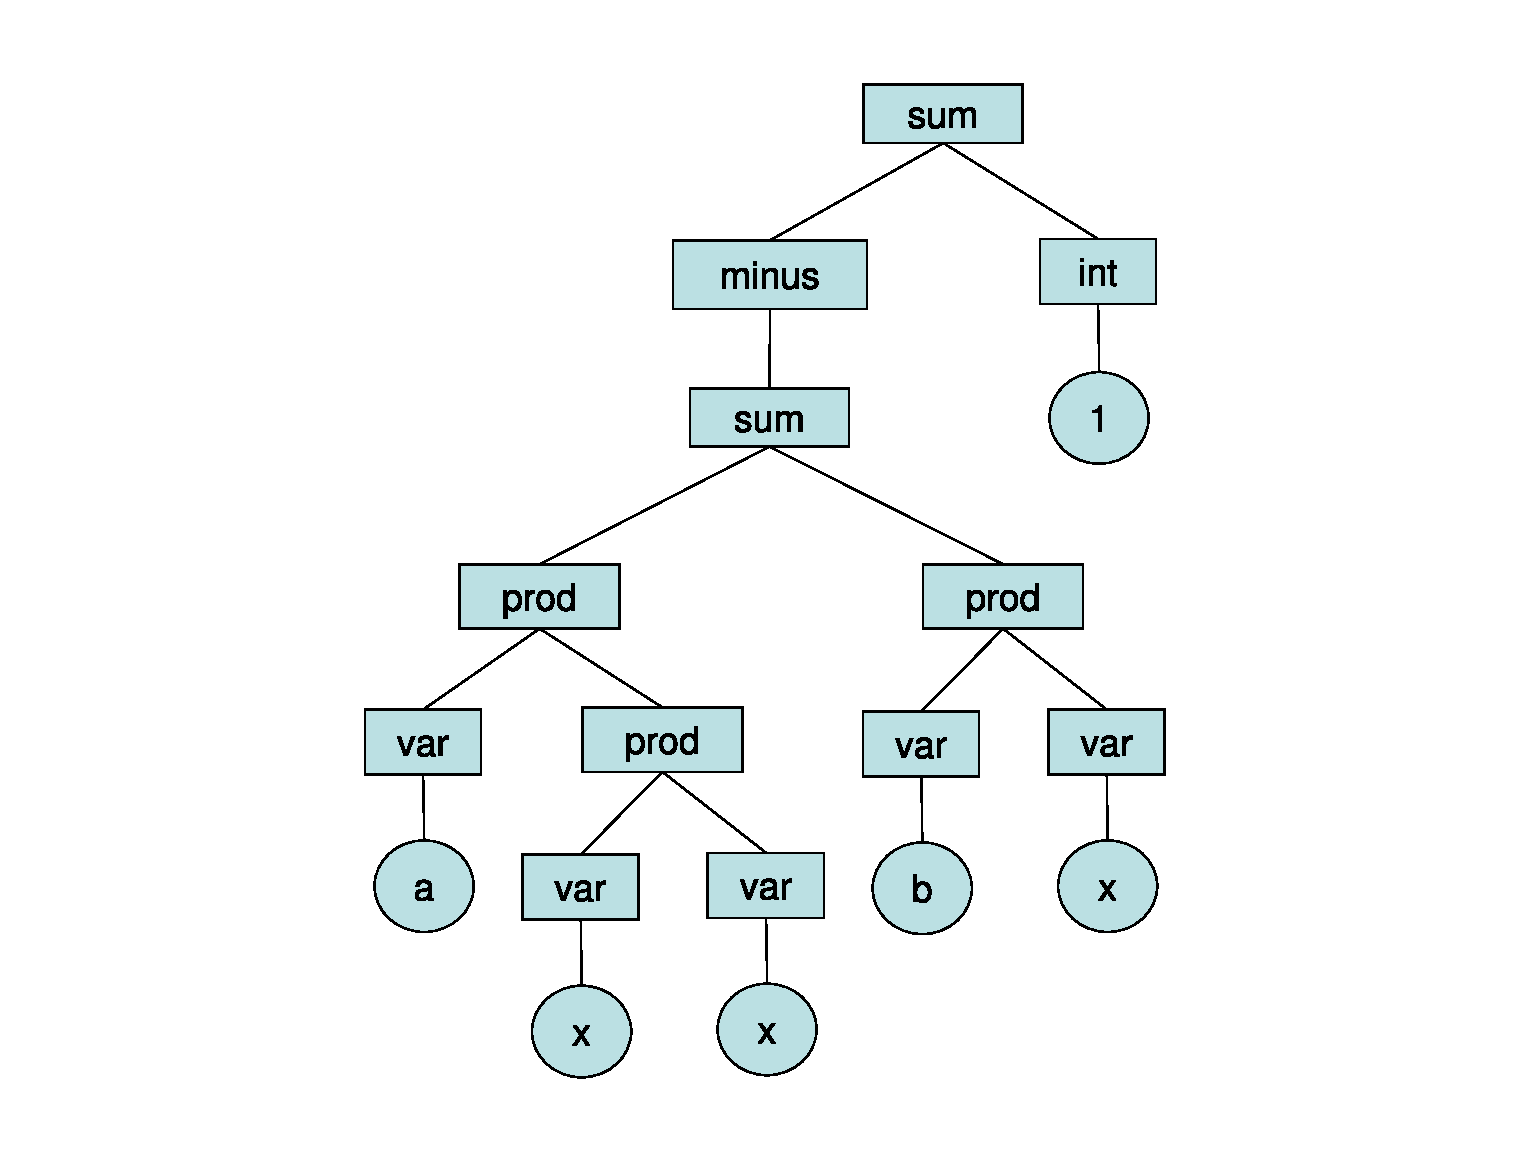
\includegraphics[width=5in]{parsetree}
\caption{Parse tree for $-(a(x\cdot x)+ bx) + 1$.}
\label{fig:parse}
\end{figure}

In a computer, such a tree would be represented by pairs or triples
that begin with a
\emph{tag} equal to the label of the top node of the parse tree.  
The general definition of parse trees for $\aexp$'s would be:

%\newcommand{\paexp}{\text{Aexp-parse-tree}}

\begin{definition}\label{arithparse}
The set $\paexp$ of \emph{parse trees for arithmetic expressions} 
over a set of
\emph{variables} $V$ is defined recursively as follows:
\begin{itemize}
\item \inductioncase{Base cases}:
\begin{enumerate}
\item If $n \in \integers$, then $\ang{\texttt{int}, n} \in \paexp$.
\item If $v \in V$, then $\ang{\texttt{var}, v} \in \paexp$.
\end{enumerate}
\item \inductioncase{Constructor cases}: if $e,e' \in \paexp$, then
\begin{enumerate}
\item $\ang{\texttt{sum}, e, e'} \in \paexp$,
\item $\ang{\texttt{prod}, e, e'} \in \paexp$, and
\item $\ang{\texttt{minus}, e} \in \paexp$.
\end{enumerate}
\end{itemize}
\end{definition}

So the $\paexp$ corresponding to formula~\ref{ax} would be:
\begin{equation}\label{axtag}
\begin{array}{rll}
\left< \right. \texttt{sum}, 
         & \left< \right. \texttt{minus},\ \ \left< \right. \texttt{sum},
               & \ang{\texttt{prod},\ \ \ang{\texttt{var},\ a},
                                     \ang{\texttt{prod},\ \
                                            \ang{\texttt{var},\ x},\
                                            \ang{\texttt{var},\ x}}},\\
                               && \left. \left. \ang{\texttt{prod},\ \
                                       \ang{\texttt{var},\ b},\
                                       \ang{\texttt{var},\ x}}
                                   \right> \right>,\\
         & \left. \left. \ang{\texttt{int},\ 1} \right> \right>
\end{array}
\end{equation}
Now the expression~\ref{ax} is certainly a lot more humanly
intelligible than~\ref{axtag}, but~\ref{axtag} is in the
representation best suited and commonly used in compiling and
processing computer programs.

\end{editingnotes}

\endinput



%% with subtrees as shown in Figure~\ref{rotate2} and values as indicated
%% by integers corresponding to those in Figure~\ref{rotate1}. 

%%  If both are depth $d+1$, then let $U$ be the one
%% with values.  If the depth of $U$ is $d+1$,
%% then it must have branches $C,D$ of depths $d,d-1$ with at least one
%% $d$.  In this case, we re-arrange as shown in (on the right below).
%% Otherwise, the depth of $U$ is $d$ and of $R$ is $d+1$, in which case
%% $R$ must in turn have a branches $V,W$ of depths $d$ or $d-1$ with at
%% least one $d$.  This is illustrated in Figure~\ref{rotate1} with
%% integer labels corresponding to the relative values of the labels of
%% these trees.
%%                                        X6                  
%%                          d+1,2  Z2             y7  d+1    
%%                               1   4        C6.6  D8     
  
%% \begin{figure}
%% \begin{verbatim}
%%                              N2                 
%%                              /\
%%                             /  \
%%                           B1   S4
%%                                /\
%%                               /  \
%%                              /    \
%%                             /      \
%%                           R3        U5
%% \end{verbatim}

%% \caption{Tree before rotation.}

%% \label{rotate1}

%% \end{figure}

%% In Figure~\ref{rotate1},
%% \begin{align*}
%% \dpth{B} & = d\\
%% \dpth{S} & = d+2,\\
%% \dpht{R} & = d+1,\\
%% \dpht{U} & = d\\
%% \dpht{V} & = d,\\
%% \dpht{W} \in  \set{d, d-1}.\\
%% \end{align*}

%% The result of the rotation is defined to be three new trees $X,Y,Z$
%% with subtrees as shown in Figure~\ref{rotate2} and values as indicated
%% by integers corresponding to those in Figure~\ref{rotate1}.  That is,
%% \begin{align*}
%% \nlbl{X}  & = \nlbl{R},\\
%% \nlbl{Y}  & = \nlbl{N}  & = \nlbl{T},\\
%% \nlbl{Z}  &= \nlbl{S},\\
%% \dpth{Y} & = d+1,\\
%% \dpth{Z} & = d+1,
%% \end{align*}

%% \begin{figure}

%% %\graphic{}

%% \begin{verbatim}
%%            X4                         X4                                     N2                 
%%            /\                         /\                                     /\                 
%%           /  \                       /  \                                   /  \                
%%          /    \                     /    \                              d  B1   S6 d+2
%%        Y2      Z6                 Y2      Z6                                   /\               
%%        /\      /\                 /\      /\                                  /  \              
%%       /  \    /  \               /  \    /  \                       d,d+1   R4   U7 d+1
%%      B1  V3  W5  U7             B1  V3  C6.5  D8                            / \                 
%% \end{verbatim}                                                             /   \                
%%                                                                          V3     W5    C6.5   D8 
%% \caption{Tree after rotation is AVL.}

%% \label{rotate2}                                                    
                                                                   
%% \end{figure}                                                       


\iffalse
Of course, the only sensible
move at this point for the first player is to choose to remove all
three stones.  In other words, the first
player chooses $\nimg{\emptystring} \in O_{\ang{3}}$ leaving the
second player to choose a Nim game in
\[
O_{\emptystring} \eqdef \emptyset.
\]
Since there is no Nim game in $O_{\emptystring}$, the second player
loses.

\[
(2, 3)
\]

\[
\set{\text{(2), (3), (1 2), (1 3), (2 2)}}
\]

\[
\set{\set{\emptyset, \text{(1)}},\ \ \set{\set{\text{(2), (1 2)}}},\ \ \set{\emptyset, \text{(1), (2)}},\ \ \set{\text{(1), (2), (1 1)}},\ \ \set{\text{(1), (3), (1 1), (1 2)}}}
\]


Now the last game
\[
\set{\text{(1), (3), (1 1), (1 2)}}
\]
expands again to
\[
\set{\set{\emptyset},\ \ \set{\emptyset, \text{(1),
      (2)}},\ \ \set{\text{(1)}},\ \ \set{\text{(1), (2), (1 1)}}}.
\]


Now the second game, 
\[
\set{\set{\text{(2), (1 2)}}}
\]
for example, expands again to
\[
\set{\set{\emptyset, \text{(1)}},\ \ \set{\text{(1), (2), (1 1)}}}
\]
\fi
